\documentclass[main.tex]{subfiles}
% \nomenclature[A]{GPR}{Ground Penetrating Radar}%

\begin{document}
\begin{appendices}
\addtocontents{toc}{\protect\setcounter{tocdepth}{0}}

\chapter{Benchmarking}
\chaplabel{benchmarking}
Before commencing the design process, benchmarking was conducted in order to gauge the capabilities of existing platforms and sensor equipment used for landmine detection. This gave an indication of the minimum requirements to be set for the project, and helped to better understand what challenges would need to be overcome.

\section{Autonomous platforms for landmine detection}
The use of a vehicle for landmine detection allows for larger areas to be scanned in a shorter period of time. Vehicles can also support greater loads than any human operator could, which means that more sensing equipment can be carried; this in turn increases sensing capability, and reduces the likelihood of false positives. If the vehicle can operate remotely or autonomously, the risk to human operators can be eliminated entirely. For these reasons, remotely controlled or autonomous platforms have become a popular tool for landmine detection. This section looks at several such platforms that are currently in operation or in development. 

%\subsection{Landmine detection vehicles}

In military scenarios, the key priority is to clear a path as quickly as possible for a convoy \parencite{portugal2014}. In many cases, landmine detection is coupled with landmine clearance. On the other hand, humanitarian demining requires greater levels of accuracy and effort. A clearance rate of 80\% is generally accepted in combat, a figure which only needs to apply to pathways where troops or convoys will travel; for humanitarian situations, the area required to be cleared is much larger, and such a low clearance is not accepted \parencite{habib2008}. \Figref{military} shows two remotely controlled landmine detection vehicles, one of which is used in military operations, while the other is commercially available for humanitarian demining.   

\begin{figure}[ht]
\centerline{
\begin{tabular}{cc}
\subfloat[FORESIGHT RDV \parencite{canada2004}]{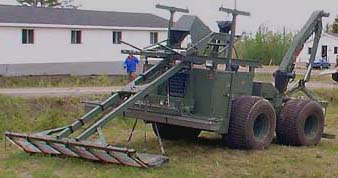
\includegraphics[height=0.25\textwidth]{8-Appendices/foresight.jpg}}
& \subfloat[NIITEK Minestalker \parencite{niitek2015}]{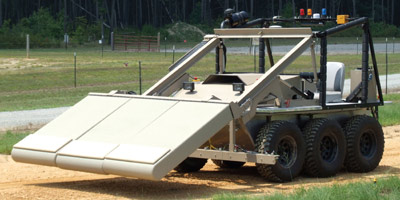
\includegraphics[height=0.25\textwidth]{8-Appendices/minestalker.jpg}} \\
\end{tabular}}
\caption{Military and commercially available vehicles for landmine detection}
\figlabel{military}
\end{figure}
 
\subsubsection*{General Dynamics FORESIGHT RDV} 
FORESIGHT is a multi-sensor landmine detection system, mounted on a vehicle that can be controlled remotely. The vehicle usually travels with a protection vehicle, which clears the the path ahead of surface-based devices, as well as mines just below the surface \parencite{canada2004}. The sensor suite consists of four independent systems, the data from which is fused to accurately detect a range of threats. A minimum metal detector array which is 3 m wide is used for the detection of metallic parts, even when the metal content is low. The 3 m GPR array with ultra-wide band capabilities (1-3 GHz) can detect larger mines at up to 30 cm below the soil surface. An infra-red camera with 8-14 micrometre wavelength is used to detect changes in soil density which occur when mines are buried \parencite{canada2004}. Finally, a thermal neutron activation detector directly detect explosives through measurements of the soil nitrogen level; this provides an added level of target confirmation \parencite{general2009}. The sensor suite can operate at a forwards speed of 3-4 km/h, and in the event that a detection is made with a sufficient confidence level, the onboard marking system is used to physically mark the threat location \parencite{canada2004}.

\subsubsection*{NIITEK Minestalker} 
Developed by the US Department of Defense and NIITEK for humanitarian demining, the Minestalker system was built to detect anti-tank mines at depths greater than 5 to 10 cm \parencite{laudato2014}. The system utilises a high performance 3.2 m VISOR GPR array and optional 3 m See-Deep metal detector array \parencite{niitek2015}. The sensors are mounted on a tractor vehicle which can be controlled remotely; the accompanying software system ensures that there is a high detection probability and a low number of false alarms. The system is a "user in the loop system", in the sense that the vehicle stops when a target is detected and waits for further instructions \parencite{laudato2014}. Targets are marked both physically and with GPS, with a 1 metre resolution. The vehicle itself can advance and detect threats in real time at up to 15 km/h \parencite{niitek2015}.

% \subsection{Research Vehicles}
% While commercially available vehicles for landmine detection are often modelled on military vehicles, research vehicles are much more varied in their design (\Figref{research}). These vehicles have been developed by universities or other research organisations, and in most cases have not seen any operational use.

% \begin{figure}[ht]
% \centerline{
% \begin{tabular}{cc}
% \subfloat[Clearpath Husky \parencite{hennessey2014}]{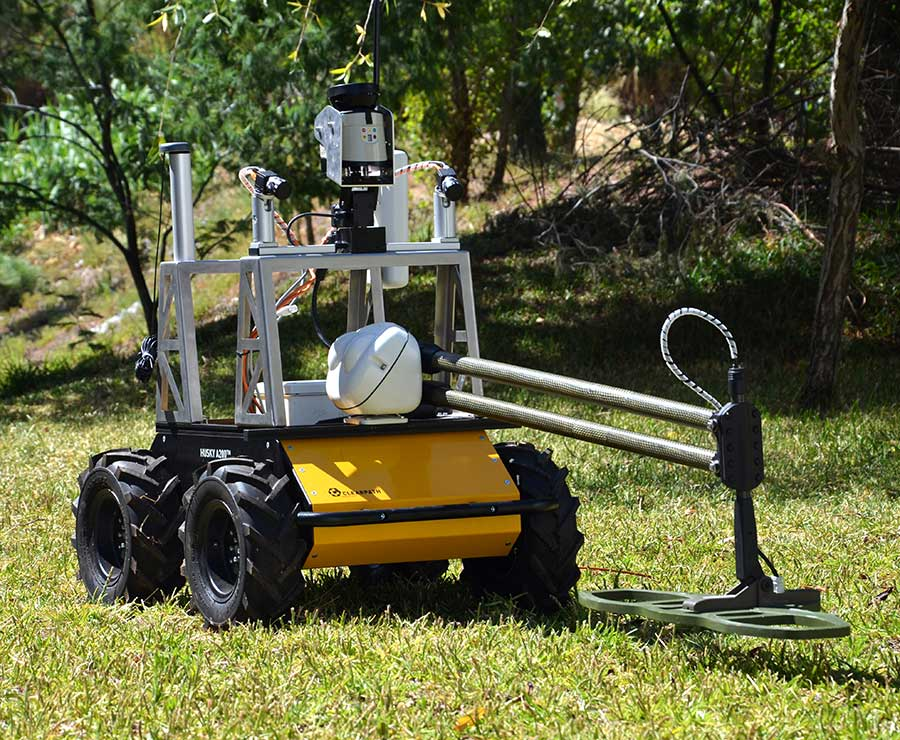
\includegraphics[height=0.3\textwidth]{8-Appendices/clearpath.jpg}} 
% & \subfloat[SILO6 \parencite{santos2007}]{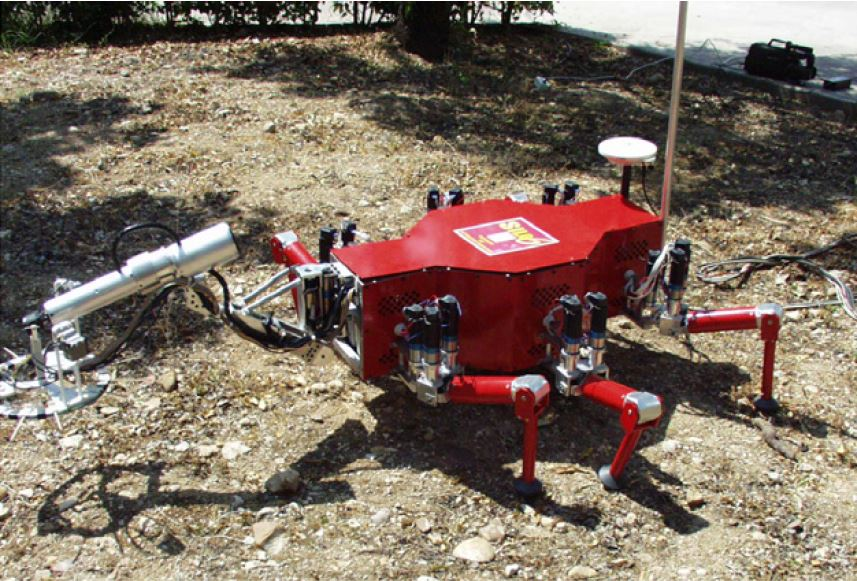
\includegraphics[height=0.3\textwidth]{8-Appendices/silo6.jpg}}\\
% \subfloat[tEODor \parencite{cubber2014}]{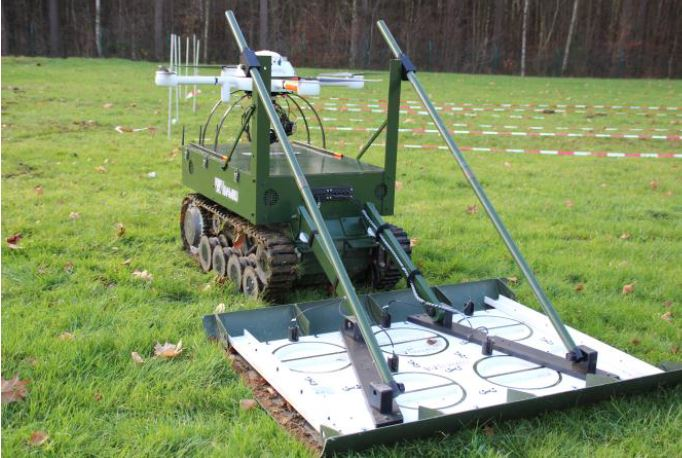
\includegraphics[height=0.3\textwidth]{8-Appendices/teodor.jpg}} 
% & \subfloat[Gryphon \parencite{fukushima2008}]{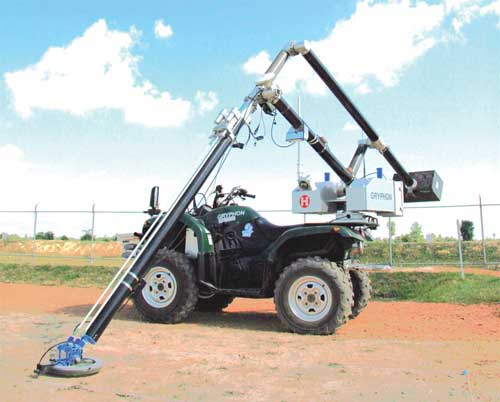
\includegraphics[height=0.3\textwidth]{8-Appendices/gryphon.jpg}}
% \end{tabular}}
% \caption{Research vehicles for landmine detection}
% \figlabel{research}
% \end{figure}

% \paragraph{Clearpath Husky} The Husky is an autonomous vehicle produced by Clearpath Robotics. In 2012, a team at the University of Coimbra (Portugal) used this platform as  foundation to create a landmine detection vehicle \parencite{hennessey2014}. The sensor suite consists of a metal detector on a robotic arm, and a GPR. The Husky itself has autonomous capabilities, meaning it can complete a mission without operator interaction \parencite{portugal2014}. The vehicle has an operational speed of 1 m/s, with an operating time, limited due by the battery life of the Husky, of 3 hours. 

% \paragraph{SILO6} SILO6 is a six-legged landmine detection robot. The six legs allow it to better traverse rough terrain, and increase mobility; in order to increase stability, the robot can lower its centre of gravity by bending its legs \parencite{santos2007}. The robot is semi-autonomous, however it has a limited sensor capability. The only sensor currently used is a Schiebel AN-19/2metal detector, which is capable of detecting objects with a low metal content. The design of the platform restricts the operating speed to 0.5 m/s, with a typical speed of 0.1 m/s, while the maximum operating time is 1 hour \parencite{portugal2014}.  

% \paragraph{tEODor} The tEDOor platform is a tracked, remotely controlled vehicle that is commercially available for the disposal of explosive ordnance. The platform was heavily modified by the Royal Military Academy (Belgium) to assist in humanitarian demining \parencite{cubber2014}. A metal detector array is fitted to the front of the platform, which is able to detect both small and large mines. The system works in conjunction with an unmanned aerial vehicle, which firstly scans the area using visual and infra-red sensors, and identifies points of interest which tEODor investigates. Being a tracked vehicle, the operating speed is limited, in this case to a maximum of 0.8 m/s, while the operating time is 203 hours \parencite{portugal2014}.   

% \paragraph{Gryphon}
% The Gryphon project is larger in scale than the rest of the research projects introduced. It uses a commercially available quad bike on which a large arm has been fitted \parencite{fukushima2008}. The length of the arm allows the vehicle to remain completely outside of the test lane, meaning this it is less susceptible to damage. A metal detector or GPR can be fitted to the end of the arm, though not at the same time. Since the platform is a larger vehicle, is can be operated at speeds of up to 5 m/s, and the petrol engine allows a 10 hour operating time \parencite{portugal2014}.  

% The various vehicles introduced show that there are many approaches to automated landmine detection, both in terms of the platforms used and the sensors available. While many solutions exist, no one method can be adapted to all scenarios, and there is much room for innovation and further research. \textcolor{red}{Need to speak about the challenges that are present}

%\section{Landmine Detection}
%There have been similar projects that have used MD, GPR or a  combination of both to achieve detection and classification of landmines or unexploded ordinances (UXO). The various models of MD, GPR will be compared in order to determine if the specific details are suitable for landmine detection and if the scenario of operations (\textcolor{red}{insert reference to scenario of operations}) are achievable based on these specifications. 

% \subsection{Metal Detectors}
% \textcolor{red}{Insert some benchmarking here that Rahul did}

% \subsection{Ground Penetrating Radar}
% \textcolor{red}{Need to relate to the scope as well, i.e. soil types and operational environments\\}
% What has been achieved with the GPR in terms of the operation environment and soil types. etc. that can be linked and based on

%In order to meet the system requirements \textcolor{red}{(insert reference to system requirements here)} and  scenarios of operation of the landmine, there are operating parameters required. The operating specifications of a GPR for landmine detection are listed as follows \textcolor{red}{insert Pasolli reference here}:
% \begin{itemize}
% \item{\textbf{frequency:} 10 MHz - 3 GHz}
% \item{\textbf{Penetration depth:} 1 cm - 3 m.}
% \item{\textbf{Surface types:} Sand, humus soil}
% \item{\textbf{Operating time:} 1 ns to 60 ns}
% \item{\textbf{No. of data scans:} 200 - 600}
% \end{itemize}

%The following comparisons of specific GPRs that may be used in landmine detection should meet or exceed the specifications above. There are various types of commercial GPRs, such as NIITEK, SIRO-Pulse, and others as provided below. %-Still changing this part. 

%\paragraph{NIITEK GPR}
%AS provided in landmi
%\paragraph{SIRO-Pulse}

%\paragraph{DX Antenna Array GPR} This type of GPR meets the operating criteria above as specified in \textcolor{red}{see appendix}. There are various applications that this GPR may be used including archaeology,

%The detection of subsurface objects is one of the main uses for a GPR. This concept may be used in various applications including landmine detection. The GPR is able to detect landmines with various types of casing. An advantage of the GPR sensor is that there are both handheld and array types which assist in both manned and unmanned landmine detection operations. There are two types of GPRs, namely pulse radar (time-domain) and frequency-domain \textcolor{red}{specific reference here}. 

%In order detect and identify the subsurface objects as mentioned in \textcolor{red}{reference objective section}, the GPR signals are required to be processed. There are various methods implemented to detect landmines using GPR \textcolor{red}{INSERT CITE}. The first part is the preprocessing of the signals in order to remove signal clutter. This is processed further in order to identify the object under the surface and minimise false positives.

%The detection and classification of landmines and subsurface objects are achieved through existing algorithms, such as, hough transformation, bayesian, feature extraction, kalman filters.   

%\textcolor{red}{NOTE: Need to mention anything commercialised here. Types of GPR used, and the operation frequency they used. The penetration depth etc. etc. Nothing too specific. Just how they've done it. Elaborate on the types in Literature review.} \textcolor{green}{perfect. this is exactly what i was going to put in here - i had a spreadsheet on the GoogleDrive with most of this data in it, but it seems to have gone walkabout}

% Need to check everything
%NOTE NO PHYSICAL MARKING OF THE LANDMINE
%It is also possible to detect the composition of the explosives used in the landmines, however, this is only used in conjunction with the electromagnetic properties returned to receive the signals. 

%Link to Challenges in identifying the landmine due to background noise etc. 
% Need to mention that a database for identification is generally difficult to achieve with regards to current mines. Limitation include that the objects have similar reflected signals, such as rocks vs composite landmines. 

% Need to talk about the usefulness of the GPR and landmine together. How they complement each other. 

\section{Capabilities of landmine detection equipment}
Current mine sweeping methods that employ handheld metal detectors achieve high rates of detection for subsurface metallic mines. The main limitations of the handheld metal detecting systems is the inability to detect mines constructed from non-metallic composite materials, and the shallow depth capabilities provided by the metal detector. These systems also have a high rate of false positives due to the inability for an operator to differentiate between mines and shrapnel fragment or other buried metal objects.

Handheld mine detection devices currently used by the ADF for military purposes include the Minelab F3 series. This device is used to clear paths for vehicles by tracking the wheelbase and scanning for anti-vehicle mines. It has a sensing depth suitable to allow the detection of almost all anti-tank and anti-personnel mines that will pose a threat to an operator, though it has the expected high rate of false positives \parencite{minelabF3}. The process for determining which items are suspicious and require excavation, and which items are unremarkable shrapnel, is required to be undertaken by a skilled operator.
\begin{figure}[ht]
\centerline{
\begin{tabular}{cc}
\subfloat[Minelab F3 \parencite{minelabF3}]{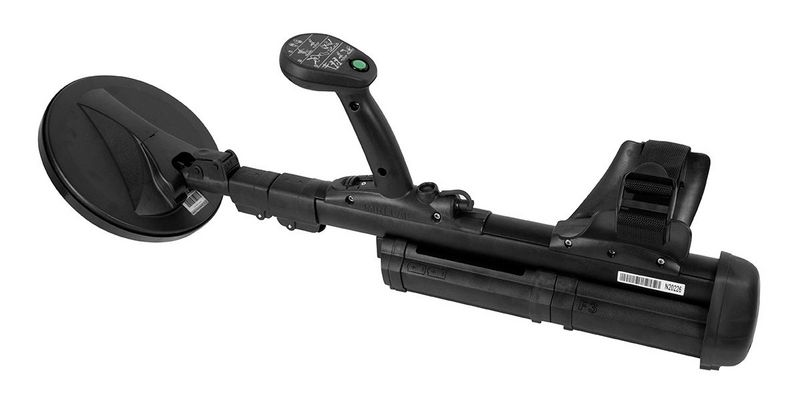
\includegraphics[width=0.5\textwidth]{8-Appendices/minelabF3.jpg}} 
& \subfloat[Minelab STMR \parencite{minelabArray}]{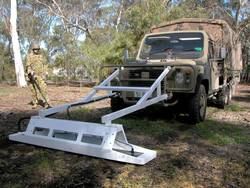
\includegraphics[width=0.4\textwidth]{8-Appendices/stmr.jpg}}\\
\end{tabular}}
\caption{Minelab metal detector systems used by the ADF \& DSTG}
\figlabel{metaldetectors}
\end{figure}

Minelab also provides the STMR, a vehicle mounted metal detection array that reduces the need for on-foot operators in front of a convoy. The sensor is capable of sampling at a rate of 200 Hz, meaning that the device can detect objects while moving at speeds up to 50 km/h \parencite{3dradarDXG}. Like the F3 series, the STMR is capable of detecting minimum-metal mines, such as the composite M14 anti-personnel mine, which contains only a small button sized metal detonator in the entire device \parencite{minelabArray}. The STMR system provides some level of feature recognition, providing a display to the operator inside the vehicle which reports scanned data \parencite{minelabArray}.

Commercially available GPR systems are commonly intended for non-mine detection purposes, such as utility and buried pipe detection. The limitations of 2D radar systems, which include the majority of available GPR devices, is that the narrow scan width means that the antenna is required to pass directly over the mine object to register a detection. A typical scan deviance from the buried object to still consistently register a detection is approximately 150 mm \parencite{3dradarDX}.

Commercial 2D GPR systems range from handheld devices which are intended to detect utilities and locate studs in wall cavities, such as the RadioDetection RD8000, have detection depths of only a few centimetres and limited resolution \parencite{rd8000}. More advanced systems with limited depth ranges, such as the US Radar Seeker 2000 HH are capable of detection resolutions to allow identification of a fishing line at depths of 0.6 metres \parencite{usradar}. The ability to consistenty locate features this small are limited by the signal to noise ratio, a property of the soil in which the search is undertaken. Typical limits for detection capabilites of these GPR units range from a few centimetres to many metres in depth, with reduced resolution as depth of scanning increases.
\begin{figure}[ht]
\centerline{
\begin{tabular}{cc}
\subfloat[RadioDetection RD8000 \parencite{rd8000}]{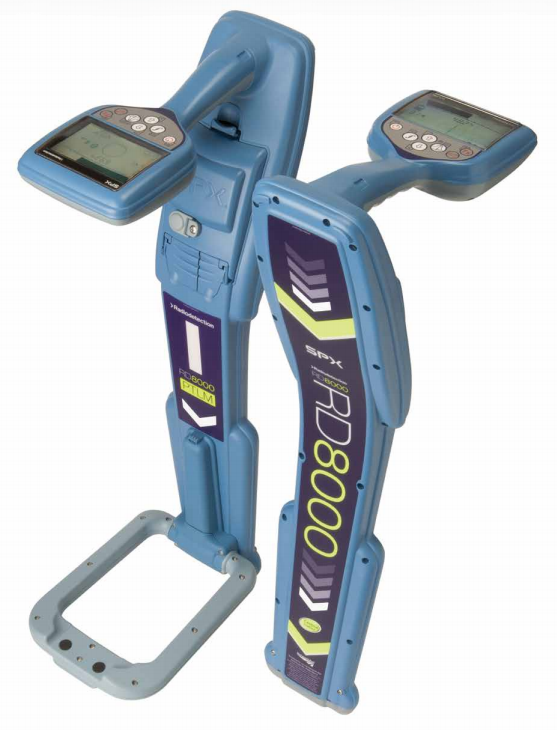
\includegraphics[height=0.4\textwidth]{8-Appendices/rd8000.png}} 
& \subfloat[US Radar Seeker 2000 HH \parencite{usradar}]{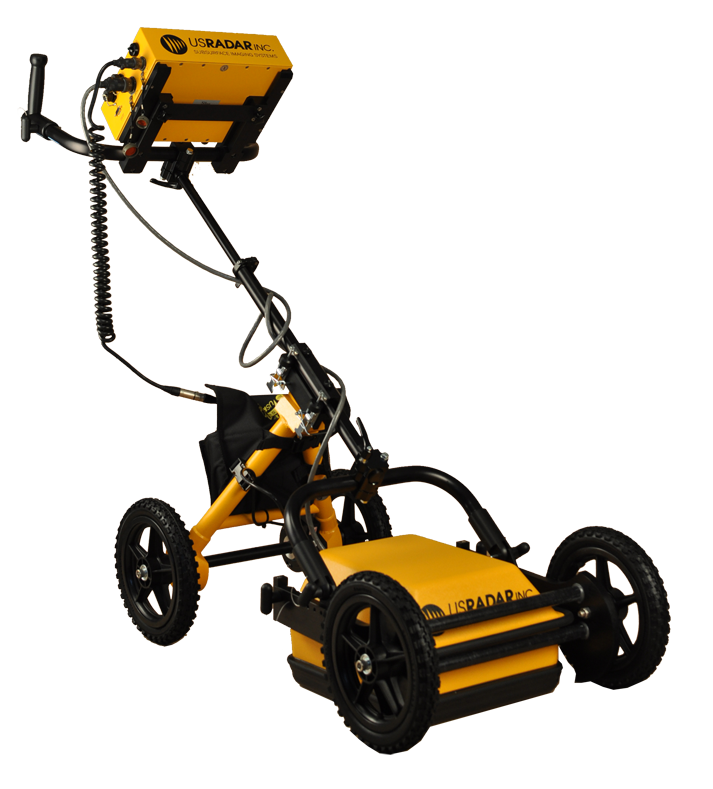
\includegraphics[height=0.4\textwidth]{8-Appendices/seeker2000.png}}\\
\end{tabular}}
\caption{Commercially available GPR systems}
\figlabel{cheapradar}
\end{figure}

A common theme among these systems is limited ability for automatic classification of targets. The large majority require a skilled operator to identify all targets and provide no degree of automatic scanning. More advanced and expensive units offer greater software capabilities for data logging and feature identification, though due to their multi-purpose nature are not capable of providing a high degree of mine detection and identification autonomously with software \parencite{rd8000}.

Current state-of-the-art GPR systems for mine detection, such as the DX and DXG series detectors from 3D-RADAR AS have significantly greater detection capacity than other GPR systems. The DX series, which are specially designed for detection of landmines and unexploded ordnance (UXO) is capable of achieving high detection rates (>95\%) of underground mines due to its high resolution. Detection of objects down to 25 mm in feature size, and at depths of over one metre is commonly achieved \parencite{3dradarDX}. The 3D arrangement of the sensors allows for a wide scanning width making it well suited for mine sweeps ahead of a vehicle. The sensor is capable of being trailer mounted and can produce useful data at speeds of up to 30 km/h \parencite{3dradarDX}.

\begin{figure}[ht]
\centering
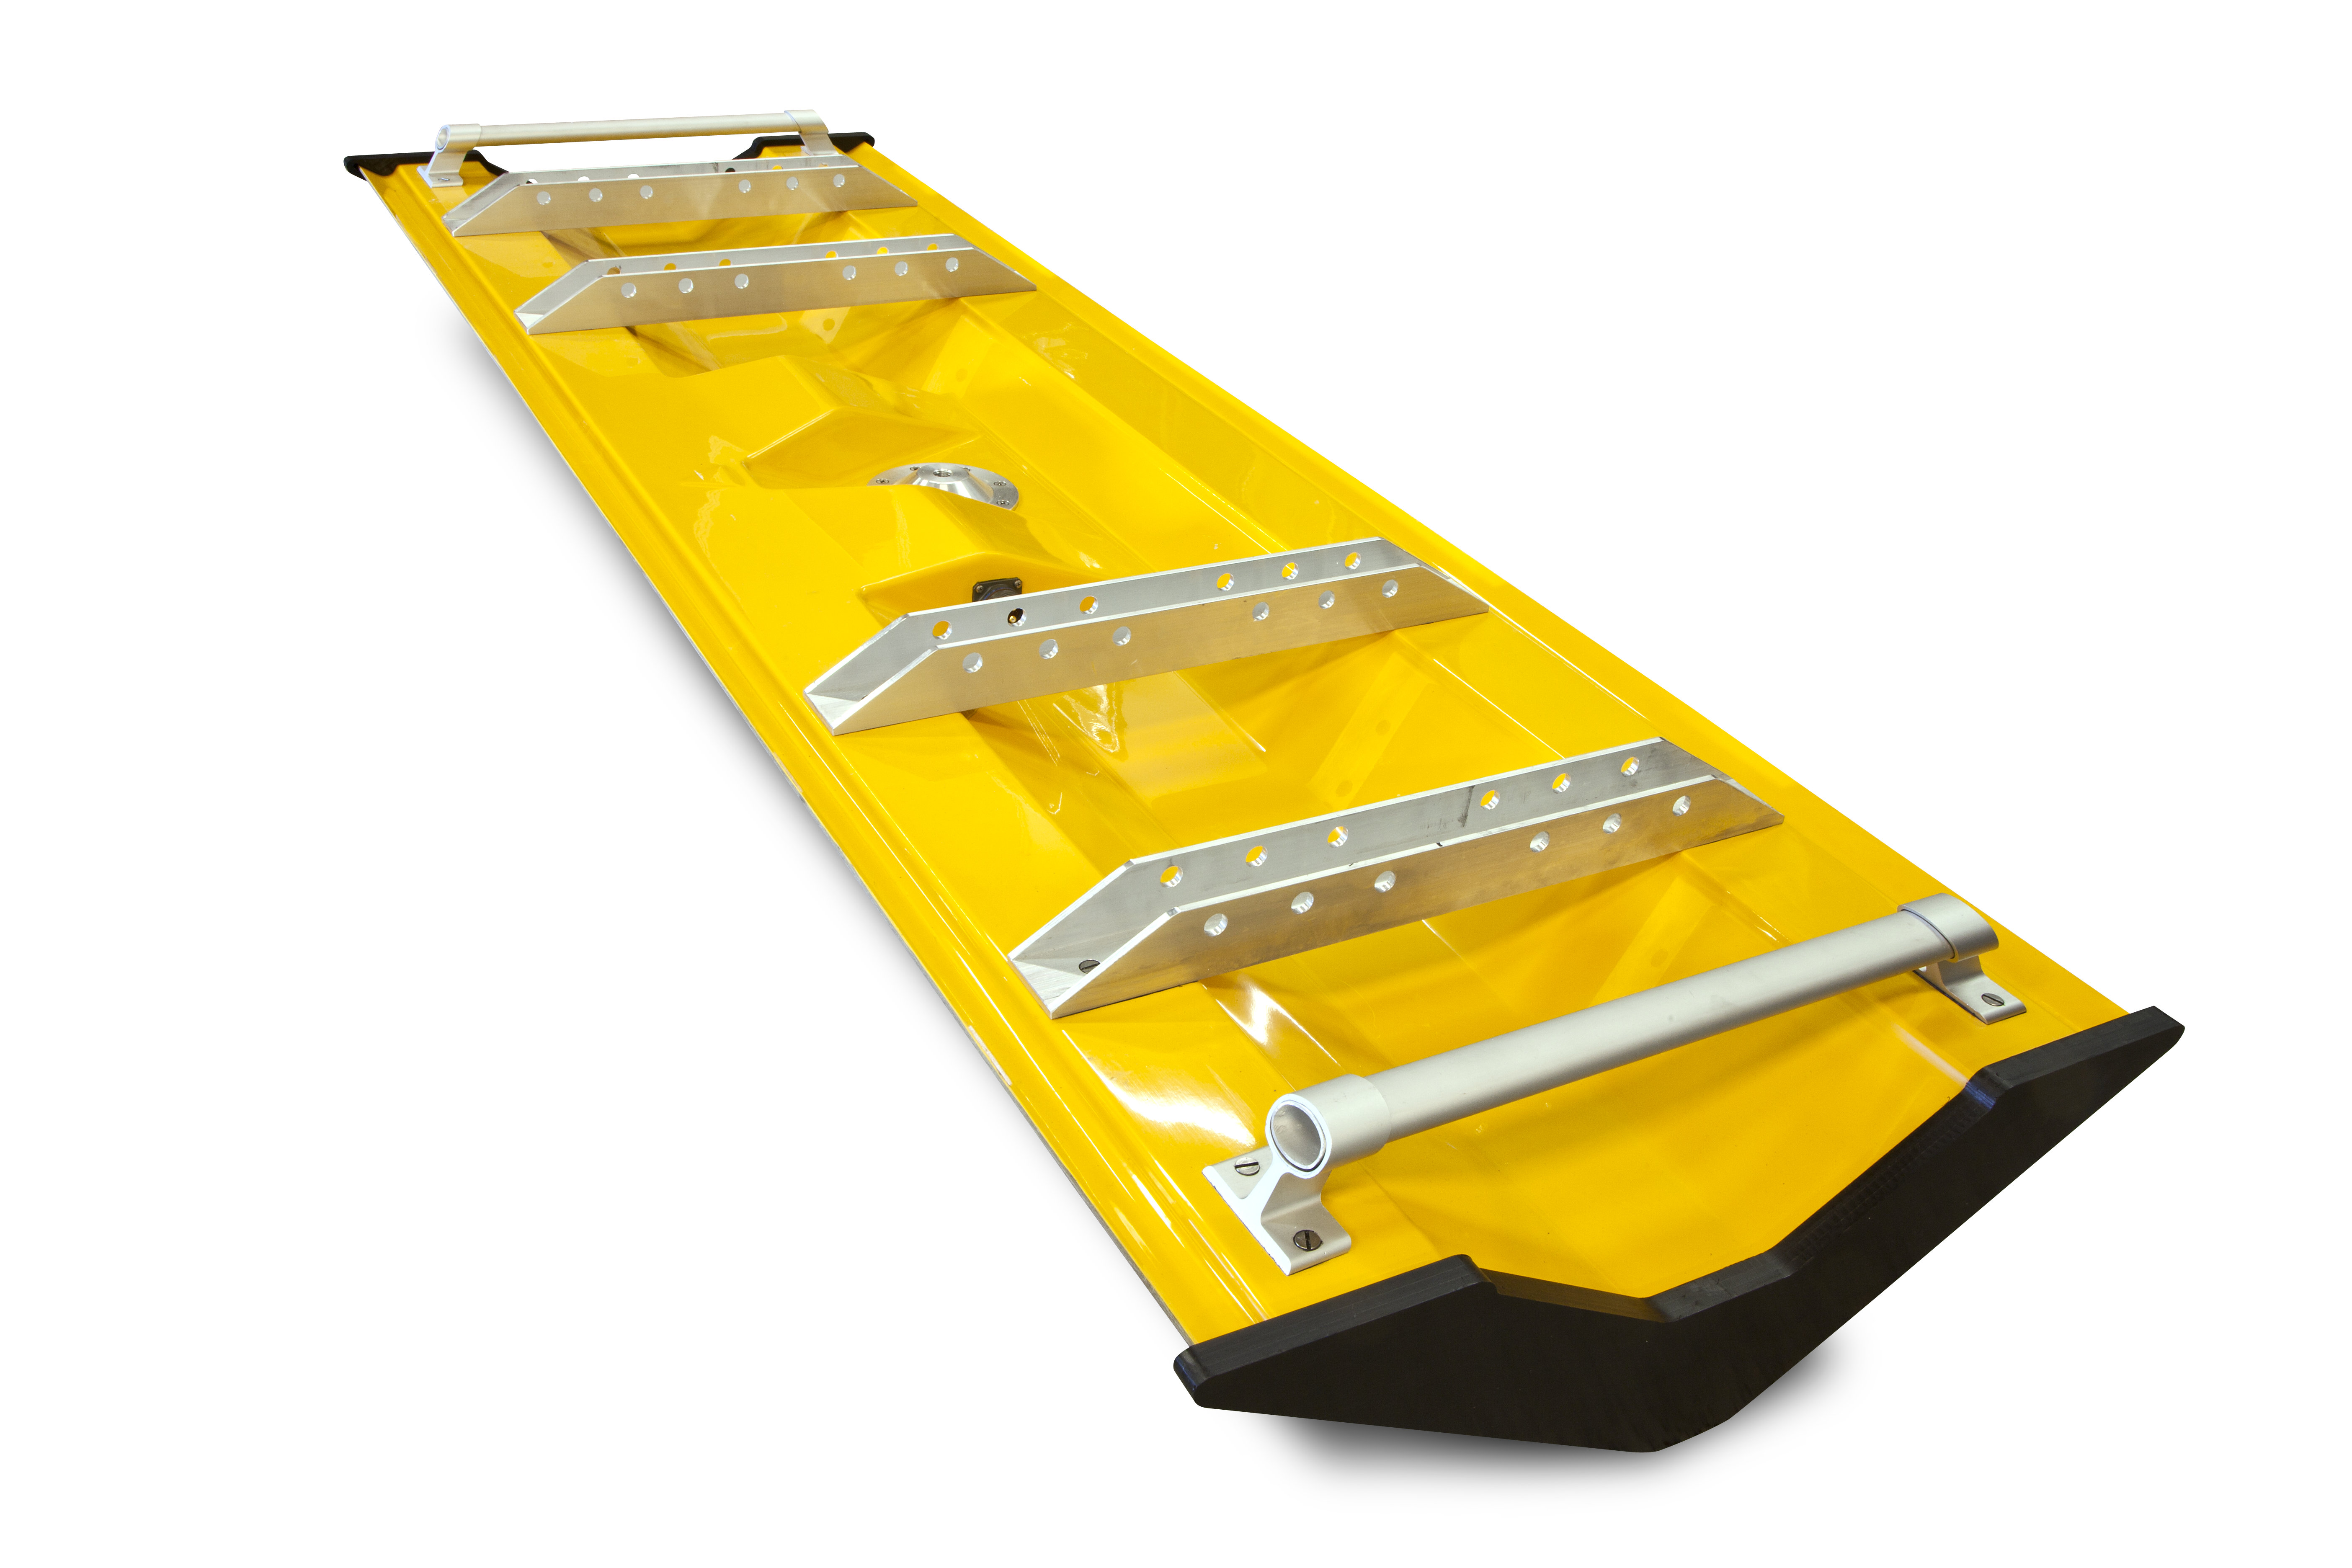
\includegraphics[width=0.55\textwidth]{8-Appendices/DX-Series-Antenna-Profile.jpg}
\caption[3D-RADAR DX series GPR antenna]{3D-RADAR DX series GPR antenna \parencite{3dradarDX}}
\figlabel{dxseries}
\end{figure}

\section*{Multisensor systems for landmine detection}
While traditional systems for landmine detection make use of a single sensor, the latest generation of systems attempt to combine multiple sensors. This allows for a broader range of threats to be detected, and at the same time increase detection accuracy.  

% There is no benchmark here so no point talking about it
%\paragraph{AN/PSS-14} The AN/PSS-14, formerly known as the Handheld Standoff Mine Detection System (HSTAMIDS), is the standard mine detector used by the US army since 2006 \parencite{L32012}. The system combines a ground penetrating radar with a metal detector and is designed to detect both anti-tank and anti-personnel mines. The wide-band GPR has a single transmit and two receive antennas, and forms the central part of the sensor head, while the metal detector coil sits around the GPR. Sensor fusion allows data from both sensors to be used in threat detection, which maximises probability of detection of the system while minimising the false alarm rate. In addition, the AN/PSS-14 system makes use of a real-time terrain model, which allows for optimal operation in varying soil conditions \parencite{L32012}. 

One such example is the Vallon Minehound, a commercially available handheld detector that combines a Vallon metal detector with a Cobham GPR \parencite{WM2016}. While the system is designed to find anti-tank and anti-personnel mines, it can also detect low metal content threats such as IEDs. 
%The metal detector employs pulse induction detection to find threats even in soils with a high mineral content, and can be used either independently or in conjunction with the GPR. 
%When used in conjunction, metallic clutter may be ignored, and non-metallic threats can be found. 
System performance in average soil condition allows for detection at depths up to 20 cm for anti-personnel and 40 cm for anti-tank mines, with an overall false alarm rate less than 25\% \parencite{daniels2005}.

Another system is being developed to allow demining and reclamation of vast swathes of currently unsafe land in rural Egypt, where remnants of World War II still pose a significant risk to local communities. The challenge of the Egyptian sands is that the frequently shifting ground surface means that mines are periodically uncovered or more deeply buried than when originally placed many decades ago \parencite{NATOnewsroom}. The system developed combines a highly sensitive metal detector, capable of recognising metallic objects buried at depths greater than a metre, with a GPR which is used to determine the shape and volume of objects located by the metal detector \parencite{NATOnewsroom}. This arrangement allows the detection of deep objects and a reduction in the rate of false positives, reducing the frequency of costly deep excavations of harmless shrapnel.


% There is no benchmark here, so no point talking about it
%\paragraph{ALIS} The Advanced Landmine Imaging System, or ALIS, is a Japanese system that can be integrated with an existing metal detector with minimum modification  \parencite{sato2005}. In addition to the audio output produced by the metal detector, ALIS produces a visual image that combines the metal detector signals with GPR images. The GPR used is a 1-3 GHz impulse radar system, and in order minimise the effect on the metal detector coils, it is mounted at the front of the system  \parencite{sato2005} The signals from both sensors are co-located through the use of a camera mounted on the system, which tracks the relative position of each one.


% Link to challenges in integration 

%The current challenges with landmine detection, including further elaboration of each signal processing methods are \textcolor{red}{reference literature review section}. 

%%%%%%%%%%%%%%%%%%%%%%%%%%%%%%%%%%%%%%%%%%%%%%%%%%%%%%%%%%%%%%%%%%%%%%%%%%%%%%%%%%

\chapter{Platform Selection}
\chaplabel{platformSelectionApp}
As stated in the concept design, the requirements for the platform are as follows: 

\begin{itemize}
 \item Payload: The platform should be able to carry a total payload of 100 kg, and must allow for this payload to be mounted.
 \item Terrain traversing: The platform should be able to travel off-road in regions with dry sandy soils and level unobstructed terrain.
\item  Operational speed and acceleration: The platform should be able travel in a straight line, both forwards and reverse, and perform turns while maintaining an operational speed of 5 km/h.
\item Manoeuvrability and controllability: The platform should be manoeuvrable enough to navigate a region of interest, with a smaller turning angle preferred, yet controllable enough that in case of an emergency, it can come to a complete stop from its operational speed in 1 m.
\item Cost and availability: The platform should have a reasonable cost given the project budget of \$16,500, ans should be available for use as early as possible. 
\item Ease of automation: The platform should be sufficiently simple to automate, with a preference given to platforms that have the framework for automation already implemented. 
\item Ease of transportation: The platform should be sufficiently easy to transport from a workshop to a testing locations using a ute or trailer.
\end{itemize}
The following selection process compares several platforms against these requirements, before selecting the most suitable one. 

\section{Utility quad bike}
Quad bikes are designed to operate off-road, and are capable of traversing a wide variety of terrains with very little difficulty. Since they are designed to carry large loads as well as a human operator, utility quad bikes frequently have load limits larger than 100 kg. The turning radius for a quad bike is typically in the range of 3-4 metres, and the braking distance is small, especially at low speeds. Commercial quad bikes can be purchased at a range of prices, however almost all fall comfortably within the budget. The DSTG also offered the use of an autonomous quad bike, which was previously developed at the University of Adelaide \parencite{scheiner2011}. This quad bike, as seen in \Figref{2011quadbike}, is a Honda TRX450r and has a payload capacity of 110 kg. The quad bike was previously fitted with remote control capabilities and is in good working condition, however \textcite{scheiner2011} recommended that some actuators and electronics should be replaced.
\begin{figure}[ht]
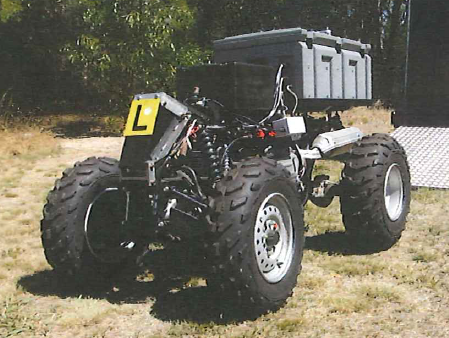
\includegraphics[width=0.5\textwidth]{8-Appendices/2011quadbike.PNG}
\centering
\caption[Autonomous quad bike offered by the DSTG]{Autonomous quad bike offered by the DSTG \parencite{scheiner2011}} \figlabel{2011quadbike}
\end{figure}

\section{Dune buggy}
A dune buggy is a vehicle designed for high speed operation on loose, sandy terrain. Dune buggies are commonly designed with an open chassis housing a modified vehicle and thus its performance characteristics are similar to or better than that of a small car. An example is the Kandi-150 shown in \Figref{kandi150}, which is built to carry two people, allowing for a load capacity exceeding 160 kg. Due to the high speeds at which these vehicles are usually operated, they have turn radii around 6 metres \parencite{150GKM}, restricting path curvature for accurate tracking. Due to the nature of the platform, it would be more expensive than a quad bike and also more difficult to automate.
\begin{figure}[ht]
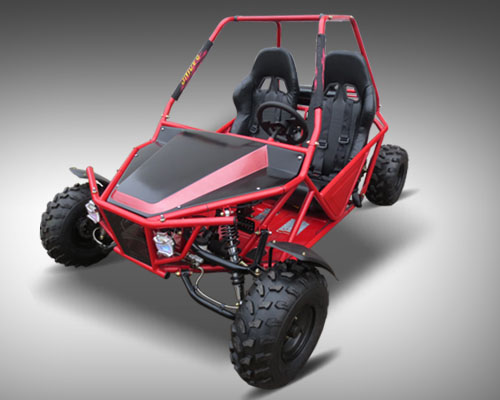
\includegraphics[width=0.5\textwidth]{8-Appendices/kandidunebuggy.jpg}
\centering
\caption[Kandi-150 dune buggy]{Kandi-150 dune buggy \parencite{150GKM}} \figlabel{kandi150}
\end{figure}

\section{Tracked vehicle}
Tracked vehicles are designed to distribute the weight of a vehicle over a large area enabling the traversing of soft and loose terrain without the concern of losing traction and becoming stuck. The platform shown in \Figref{grillon500} is one example of such a vehicle. The Grillon-500 is able to carry a payload of 1000 kg and operate at speeds up to 11 km/h \parencite{cinamGrillon}. This model is designed to support the mounting of various equipment in the front bay (fork lift pictured). An advantage of the tracked vehicle over other platforms is its ability to turn on the spot, eliminating the need for complicated turn algorithms. 
\begin{figure}[ht]
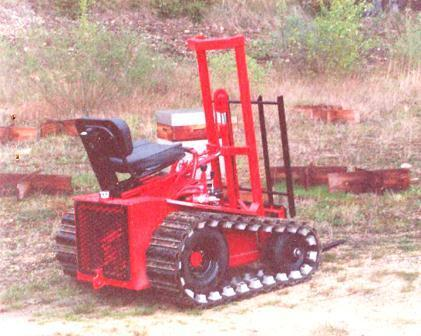
\includegraphics[width=0.5\textwidth]{8-Appendices/Grillon-500.jpg}
\centering
\caption[Grillon-500 tracked vehicle]{Grillon-500 tracked vehicle \parencite{cinamGrillon}} \figlabel{grillon500}
\end{figure}

\section{Hovercraft}

The final platform considered was an existing hovercraft from a University of Adelaide honours project in 2009. Analysis of the technical report \parencite{hovercraft2009} and experimental and theoretical evaluations showed that the lift fan was able to support a payload of up to 22 kg and the thrust fans were only just capable of moving the craft on a flat, smooth surface. Furthermore, it was expected that vibrations produced through the lift and thrust systems on hovercraft platforms would be detrimental to the effectiveness of the sensor equipment. For complete automation, only actuators for the lift motor would be required as remote operation for the thrust system had already been implemented. The stopping distance was lacking due to the time required to rotate fans for reverse thrust. The hovercraft had an advantage over other platforms through its ability to pass directly over a landmine without detonation occurring, however, this 'sliding' advantage introduces new problems when developing a path tracking algorithm due to the advanced dynamics of the platform. This 'sliding' is also a disadvantage is the hovercraft passes over a landmine without detecting it, since it place demining personnel at risk.
\begin{figure}[ht]
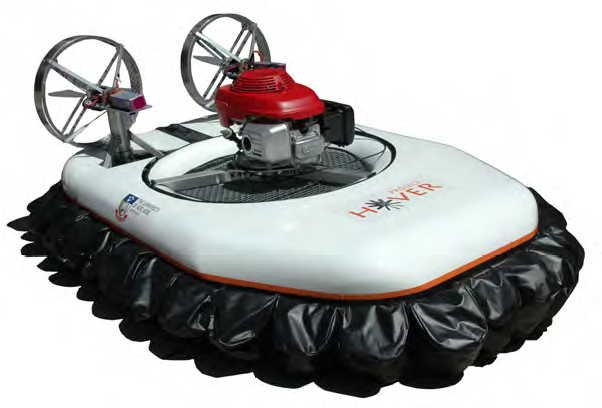
\includegraphics[width=0.65\textwidth]{8-Appendices/HovercraftPic.png}
\centering
\caption[University of Adelaide hovercraft from 2009]{University of Adelaide hovercraft from 2009 \parencite{hovercraft2009}} \figlabel{hovercraftPic}
\end{figure}

\section{Platform decision matrix}
\Tabref{platformDecision} ranks the considered platforms against the platform requirements. The hovercraft was not included due to its inability to meet the minimum payload requirement and poor manoeuvrability. A score of 10 indicates that a certain requirement has been met completely, with lower scores indicating the platform only meets the requirement to a certain extent. 

\begin{table}[ht]
\centering
\caption{Platform decision matrix}
\tablabel{platformDecision}
\begin{tabular}{r *5c}
    \multicolumn{1}{r}{}  & \mcrot{1}{l}{45}{Commercial quad bike} & \mcrot{1}{l}{45}{Dune buggy} & \mcrot{1}{l}{45}{Tracked vehicle} & \mcrot{1}{l}{45}{DSTG quad bike}\\ \toprule 
    Payload & 8 & 7 & 8 & 8\\ 
    Terrain traversing & 9 & 9 & 9 & 9\\ 
    Operational speed and acceleration & 8 & 7 & 10 & 8\\ 
    Manoeuvrability and controllability & 7 & 6 & 9 & 7\\ 
    Cost and availability & 6 & 5 & 4 & 10\\ 
    Ease of automation & 4 & 4 & 5 & 8\\ 
    Ease of transportation & 7 & 7 & 5 & 7\\ \midrule
    \textbf{Total} & 70\% & 64\% & 71\% & 81\%\\ \bottomrule
\end{tabular}
\end{table}

A commercial quad bike or dune buggy could have been used with some modifications to the structure, however a tracked vehicle or the quad bike offered by the DSTG were the two most suitable options. Of these, the tracked vehicle had superior performance specifications, however the DSTG quad bike had the advantage of direct availability at no cost, and an easier path to full automation. Hence, the DSTG quad bike was chosen as the platform for the project. 

%%%%%%%%%%%%%%%%%%%%%%%%%%%%%%%%%%%%%%%%%%%%%%%%%%%%%%%%%%%%%%%%%%%%%%%%%%%%%%%%%%

\chapter{Sensor Mount Material Selection}
\chaplabel{sensorMaterialsApp}
A formal material selection process is undertaken to find the most suitable material for the sensor mount frame, as outlined in \emph{Materials Selection in Mechanical Design} \parencite{Ashby11}. 

\section{Material index derivation}
The first step is to define the problem and find the relevant material index.

\begin{itemize}
\item \textbf{Function}: The sensor mount frame must support loads with negligible deflection and vibration.
\item \textbf{Non-negotiable constraints}: The material used must be non-metallic due to the requirements of the metal detector, and the  frame must have a minimum length $L$, to ensure the sensors are sufficiently far away from the platform.
\item \textbf{Negotiable constraints}: The frame must have a minimum stiffness $E$ equivalent to that of a metal, i.e. stiffness greater than 10 GPa \parencite{Ashby11}, good damping properties, and a suitable appearance.
\item \textbf{Objectives}: Minimise mass and vibrations.
\item \textbf{Free variables}: Cost, cross sectional area $A$.
\end{itemize}

The mass $m$ of the frame, assuming a single cantilever beam, is given by $m=AL\rho$, where $\rho$ is the material density. 

For an end loaded cantilever, the bending stiffness $k=\frac{3EI}{L^3}$, where $I$ is the moment of inertia. For a beam with a uniform square cross-section, $I=\frac{A^2}{12}$, which means that $k=\frac{3EA^2}{12L^3}$.

Rearranging and substituting into the mass equation, 
\begin{align}
m=\sqrt{3k}L^{5/2}\big(\frac{\rho}{E^{1/2}}\big).	\eqlabel{mass}
\end{align}

From this equation we can see that to minimise the mass of the frame, we have to maximise $E^{1/2}/\rho$. This material index matches that prescribed by \textcite{Ashby11} for vibration limited designs with length and beam stiffness specified.  

\section{Material selection charts}
Using this material index, material selection charts can be used to identify suitable materials. \Figref{modulus} shows a modulus-density chart, with the dotted lines indicating the stiffness limit of 10 GPa and the minimum mass guideline corresponding to the $E^{1/2}/\rho$ material index. 
\begin{figure}[ht]
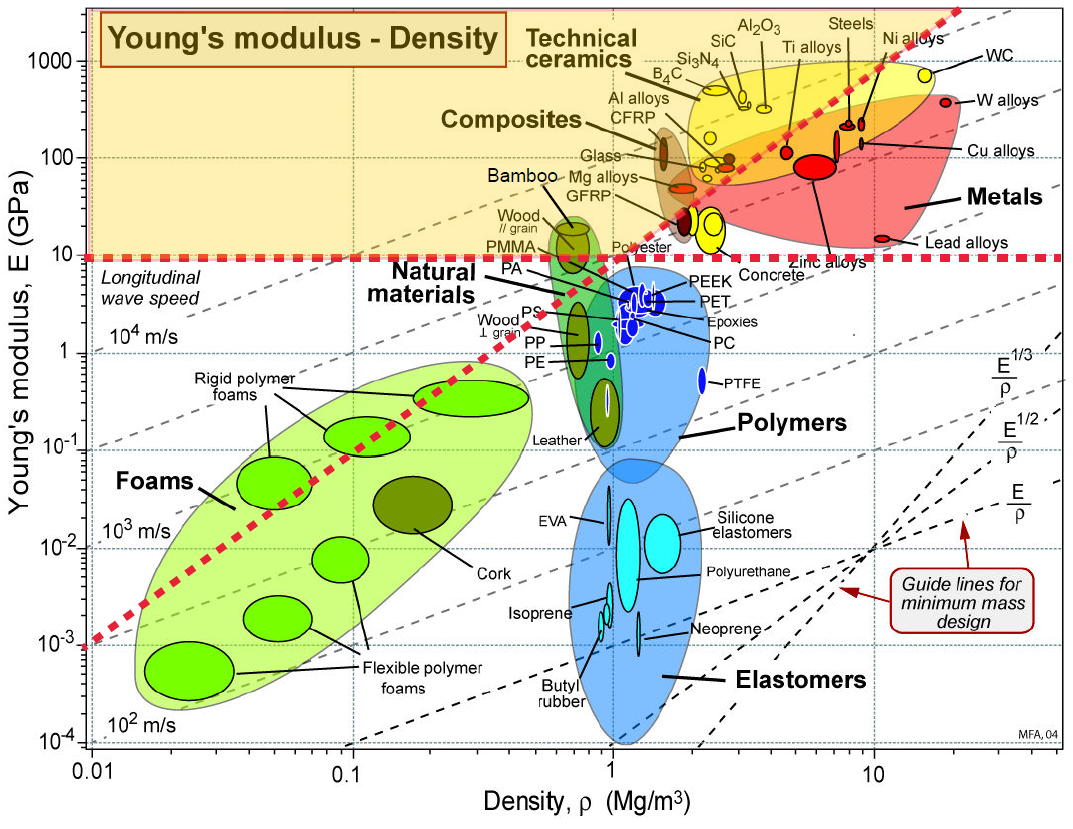
\includegraphics[width=0.9\textwidth]{8-Appendices/modulus.PNG}
\centering
\caption[Modulus-density material selection chart]{Modulus-density material selection chart \parencite{Ashby11}} \figlabel{modulus}
\end{figure}

By shifting the guideline upwards and to the left, the only materials left in the shaded region are some technical ceramics, composites, natural materials and a few metals.
\begin{itemize}
\item Metals: Magnesium and aluminium alloys lie within the region of interest, however they do not meet the non-metallic constraint.
\item Ceramics:  Several ceramic materials such as Al$_2$O$_3$, SiC, and B$_4$C have good stiffness but are heavy and quite difficult to form on account of being brittle. They are also likely to have poor vibrational characteristics.
\item Composites: Carbon and glass fibre reinforced polymers (CFRP and GFRP) have good overall properties, but are expensive and somewhat difficult to form.
\item Natural materials: Bamboo and wood (parallel to grain) also has good properties, they are light but not as stiff as other materials.
\end{itemize}
The most suitable materials are therefore natural materials including wood and bamboo, and composites including CFRP and GFRP.

\Figref{loss} shows a loss coefficient-modulus chart. Of the materials selected previously, bamboo has the highest loss coefficient, followed by wood, GFRP and CFRP, which means it has better stiffness and damping properties. 
\begin{figure}[ht]
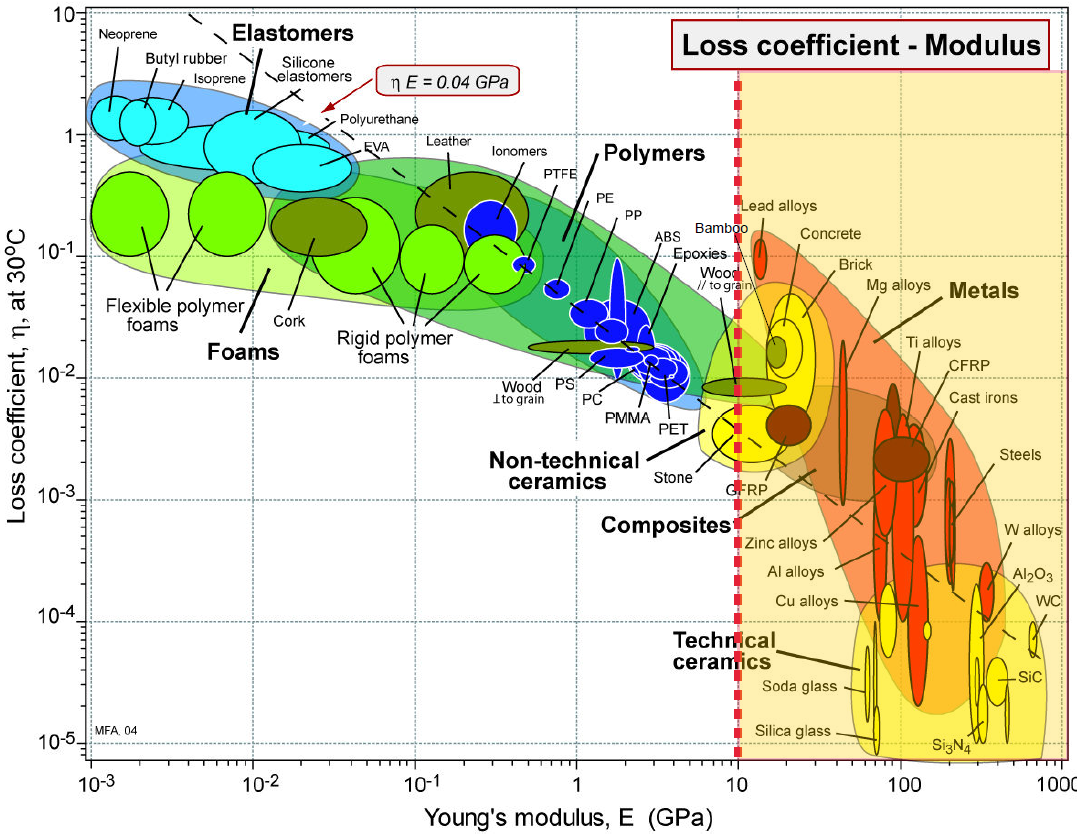
\includegraphics[width=0.9\textwidth]{8-Appendices/loss.PNG}
\centering
\caption[Loss coefficient-modulus material selection chart]{Loss coefficient-modulus material selection chart \parencite{Ashby11}} \figlabel{loss}
\end{figure}

While bamboo is the best material to use for the sensor mount frame based on loss coefficient and stiffness alone, it is difficult to obtain in Australia in structural form. Wood is the next best option, and is very easy to work with and readily available. GFRP has a similar stiffness to wood but with worse damping properties and a higher density. On the other hand, CFRP has a much better stiffness however it sacrifices damping properties and density. The two composites are also more difficult to work with, and are more expensive. Hence, the selected material is wood.

%%%%%%%%%%%%%%%%%%%%%%%%%%%%%%%%%%%%%%%%%%%%%%%%%%%%%%%%%%%%%%%%%%%%%%%%%%%%%%%%%%

\chapter{Path Subdivision Detail}
\chaplabel{pathSubdivisionDetail}
The path subdivision algorithm cycles through the user or region defined path completing two stages of subdivision at each point.
\begin{enumerate}
\item Subdivide the straight line segment up to the next point
\item If there is a following line segment, conduct a turn and align with it
\end{enumerate}
For the point $P_1 = (x_1, y_1)$, we first subdivide the line segment to the next point $P_2 = (x_2, y_2)$, shown in step 2 of \figref{simpleTurnProgression}. This is done by doing a linear interpolation between the two points to find a series of intermediate waypoints $P_i = (x_i, y_i)$:
\begin{align*}
P_i = |P_2 - P_1| \times k \times j
\end{align*}
where $k$ is the distance between intermediate waypoints and j is incremented from 0 to completion of the line segment.
\begin{figure}[ht]
\centering
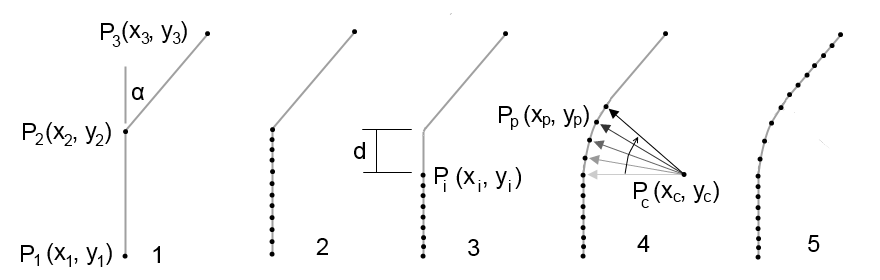
\includegraphics[width=0.9\textwidth]{8-Appendices/simpleTurnProgression.png}
\caption[Simple turn progression]{Simple turn progression}
\figlabel{simpleTurnProgression}
\end{figure}
For a simple turn, a number of intermediate points from the first line subdivision are removed up to a distance $d$ from the turn point, $P_2$. Where
\begin{align*}
d = R \tan \frac{\phi}{2}
\end{align*}
from \secref{turningspecifiedangle}. The centre point of the turn circle can then be found based on the last intermediate waypoint, $P_i$, and a vector perpendicular to the current path segment with a length equal to the turn radius, 3.14m. The vector is then incrementally rotated around $P_c$ to give the correct distance between waypoints. The required change in rotation angle at each increment is given by the following formula:
\begin{align*}
\Delta angle = \frac{distance\ between\ turn\ waypoints}{turn\ radius} = \frac{0.2}{3.14} = 0.064\ rads
\end{align*}
Incrementing stops once the vector has been rotated by a total angle equal to $\phi$. The subdivision process then continues from stage 1, by linearly subdividing the path from $P_2$ to $P_3$.

In the event of a large turn angle where an N-point turn is required, only stage 2 of the subdivision process is changed. Once the linear interpolation of waypoints is complete, some waypoints are either added or removed to the end of the line segment to aid in the alignment of the turn with the next line segment. 
\begin{figure}[ht]
\centering
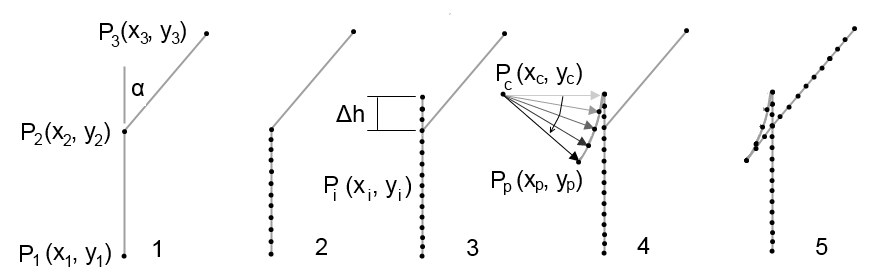
\includegraphics[width=0.9\textwidth]{8-Appendices/nPointTurnProgression.png}
\caption[Simple turn progression]{N-point turn progression}
\figlabel{nPointTurnProgression}
\end{figure}
The distance added or removed, $\Delta h$, is based on the turn angle and is found from the geometrically determined template, \tabref{npointTurnTemplate}, shown below.
\begin{table} [ht]
\centering
\begin{tabular} {r | c c c c c c c c}
Turn point & 0 & 1 & 2 & 3 & 4 & 5 & 6 & 7 \\ \hline
Heading (\degree) & 0 & 26.7 & 60.5 & 77.3 & 95.6 & 113.9 & 130.8 & 180 \\
$\Delta h$ required (m) & 0 & 1.46 & 0.09 & 0.44 & 0.37 & 0.11 & 0.62 & -1.18 \\
\end{tabular}
\end{table}
Similar to the simple turn, the centre point, $P_c$, of the turn arc is be found based on the turn radius, $R$, and is perpendicular to the current line segment. Arc points are added by incrementing the vector by the angle, $\Delta angle$. Incrementing stops once the vector has been rotated by a total angle equal to the difference between the current turn point and the next turn point, in the case of \figref{nPointTurnProgression} part 4, we are at the first turn point so the vector is rotated, $(26.7 - 0)\degree = 26.7\degree$, in total. If at this point the desired turn angle has not been reached, additional arcs are added to the path in the same fashion as just described. Stage 1 is then executed again for the next straight line segment.

\chapter{Sensor Mount Vibrations Analysis}
\chaplabel{sensorVibesApp}

\chapter{Software Design Documents}
\chaplabel{designDocs}

\chapter{Testing Procedures}
\chaplabel{testProcs}

\chapter{Sensor Test Results}
\chaplabel{sensorResults}

\chapter{Gear Actuator Truth Table}
\chaplabel{gearTable}

\chapter{Work Breakdown Structure}
\chaplabel{WBS}
The work breakdown structure shows how the technical workload of the project has been broken down into different  subsystems, and who has been assigned responsibility for managing each task. 

{\setstretch{1.15}
\begin{enumerate}
\item \textbf{Platform}\\
The platform subsystem comprises of the vehicle used to mount the sensor payload, the hardware required for automation and the physical landmine marking system. This subsystem is linked to the subsystems 3 (sensor mounting structure) and 4 (platform automation software).
	\begin{enumerate}[label*=\arabic*.]
	\item Benchmarking and literature review of platform (Harrison, Rahul)
    \item Develop specifications (Harrison, Peter)
    \item Concept designs and evaluation (Harrison, Peter)
	\item Platform evaluation and testing
    	\begin{enumerate}[label*=\arabic*.]
		\item Brake actuation (Harrison, Peter)
        \item Steering actuation (Harrison, Peter)
        \item Gears actuation (Harrison, Peter)
        \item Throttle actuation (Harrison, Peter)
        \item Platform testing (All)
        \end{enumerate}
    \item Physical landmine marking
    	\begin{enumerate}[label*=\arabic*.]
		\item Benchmarking and literature review (Jono, Racquel, Rahul)
        \item Concept designs and evaluation (Jono, Racquel, Rahul)
        \item Detailed design (Jono, Racquel, Rahul)
        \item Manufacture (Jono, Racquel, Rahul)
        \item Testing (All)
        \end{enumerate}
    \item Subsystem integration (All)
    \item Testing of integrated systems
    	\begin{enumerate}[label*=\arabic*.]
		\item Initial system testing (All)
        \item Field testing (All)
        \end{enumerate}
	\end{enumerate}
    
\item \textbf{Sensor system}\\
The sensor system includes the physical sensors that are used for landmine detection. This subsystem is linked to the subsystems 3 (sensor mounting structure) and 6 (landmine detection software).  
	\begin{enumerate}[label*=\arabic*.]
	\item Literature review on landmine detection methods
    	\begin{enumerate}[label*=\arabic*.]
        \item Metal detectors (Racquel)
        \item Ground penetrating radar (Jono)
        \item Other
		\end{enumerate}
    \item Evaluation of sensors provided by DSTG
	    \begin{enumerate}[label*=\arabic*.]
		\item Metal detector array (Jono, Racquel, Rahul)
        \item GPR (Jono, Racquel, Rahul)
        \end{enumerate}
    \item Sensor/platform integration (Harrison, Jono, Racquel)
    \item Process and interpret sensor output (Jono, Racquel)
    \item Testing (All)
    \end{enumerate}
    
\item \textbf{Sensor mounting structure}\\
The sensor mount subsystem allows the sensor payload to be mounted on the platform. This subsystem is linked to the subsystems 1 (platform) and 2 (sensor system).
	\begin{enumerate}[label*=\arabic*.]
	\item Benchmarking and literature review (Harrison, Rahul)
    \item Develop specifications (Harrison, Peter)
    \item Concept designs and evaluation (Harrison, Peter)
    \item Detailed design (Harrison, Peter)
    \item Manufacture (Harrison)
    \item Testing (Jono, Racquel, Rahul)
    \end{enumerate}
    
\item \textbf{Platform automation software}\\
The platform automation software allows the platform to operate without user input. This subsystem is linked to subsystems 1 (platform) and 5 (platform navigation software).
    \begin{enumerate}[label*=\arabic*.]
    \item Software requirements specifications (Jono)
    \item Software design document (Jono)
    \item Formulate development and testing methodology (Jono, Rahul)
    \item Primary development phase and evaluation (Jono)
    \item Secondary phase and evaluation (Jono, Rahul)
    \item Testing (Jono, Rahul)
    \end{enumerate}
    
\item \textbf{Platform navigation software}\\
The platform navigation software allows the autonomous platform to navigate a course without user input. This subsystem is linked to subsystems 4 (platform automation software) and 7 (application software). 
    \begin{enumerate}[label*=\arabic*.]
    \item Software requirements specifications (Harrison)
    \item Software design document (Harrison, Jono)
    \item Formulate development and testing methodology (Harrison, Jono)
    \item Primary development phase and evaluation (Harrison, Jono, Rahul)
    \item Secondary phase and evaluation (Jono)
    \item Testing (Jono, Racquel, Rahul)
    \end{enumerate}
    
\item \textbf{Landmine detection software}\\
The landmine detection software processes signals from the sensor system in order to detect landmines. This subsystem is related to subsystems 2 (sensor system) and 7 (application software).
    \begin{enumerate}[label*=\arabic*.]
    \item Software requirements specifications (Jono, Racquel)
    \item Software design document (Jono, Racquel)
    \item Formulate development and testing methodology (Jono, Racquel)
    \item Primary development phase and evaluation (Jono, Racquel, Rahul)
    \item Secondary phase and evaluation (Jono, Racquel, Rahul)
    \item Testing (Jono, Racquel, Rahul)
    \end{enumerate}
    
\item \textbf{Application software}\\
The application software allows an operator to remotely view the progress of the platform while it searches for landmines. This subsystem is linked to subsystems 5 (platform navigation software) and 6 (landmine detection software).
    \begin{enumerate}[label*=\arabic*.]
    \item Selection of control device (Jono)
    \item Software requirements specifications (Jono)
    \item Software design document (Jono)
    \item Formulate development and testing methodology (Jono)
    \item Primary development phase and evaluation (Jono)
    \item Secondary phase and evaluation (Jono)
    \item Testing (Jono, Racquel, Rahul)
    \end{enumerate}
\end{enumerate}}

\chapter{Gantt Chart}
\chaplabel{ganttChart}
The Gantt chart provides an overview of the timeline for the entire project. Major tasks are listed, as well as key milestones and deliverables. Tasks are assigned to team members, and progress on tasks is monitored at weekly meetings. The Gantt chart that was provided with the project charter, and the most up-to-date version of the Gantt chart, are both included on the following pages.
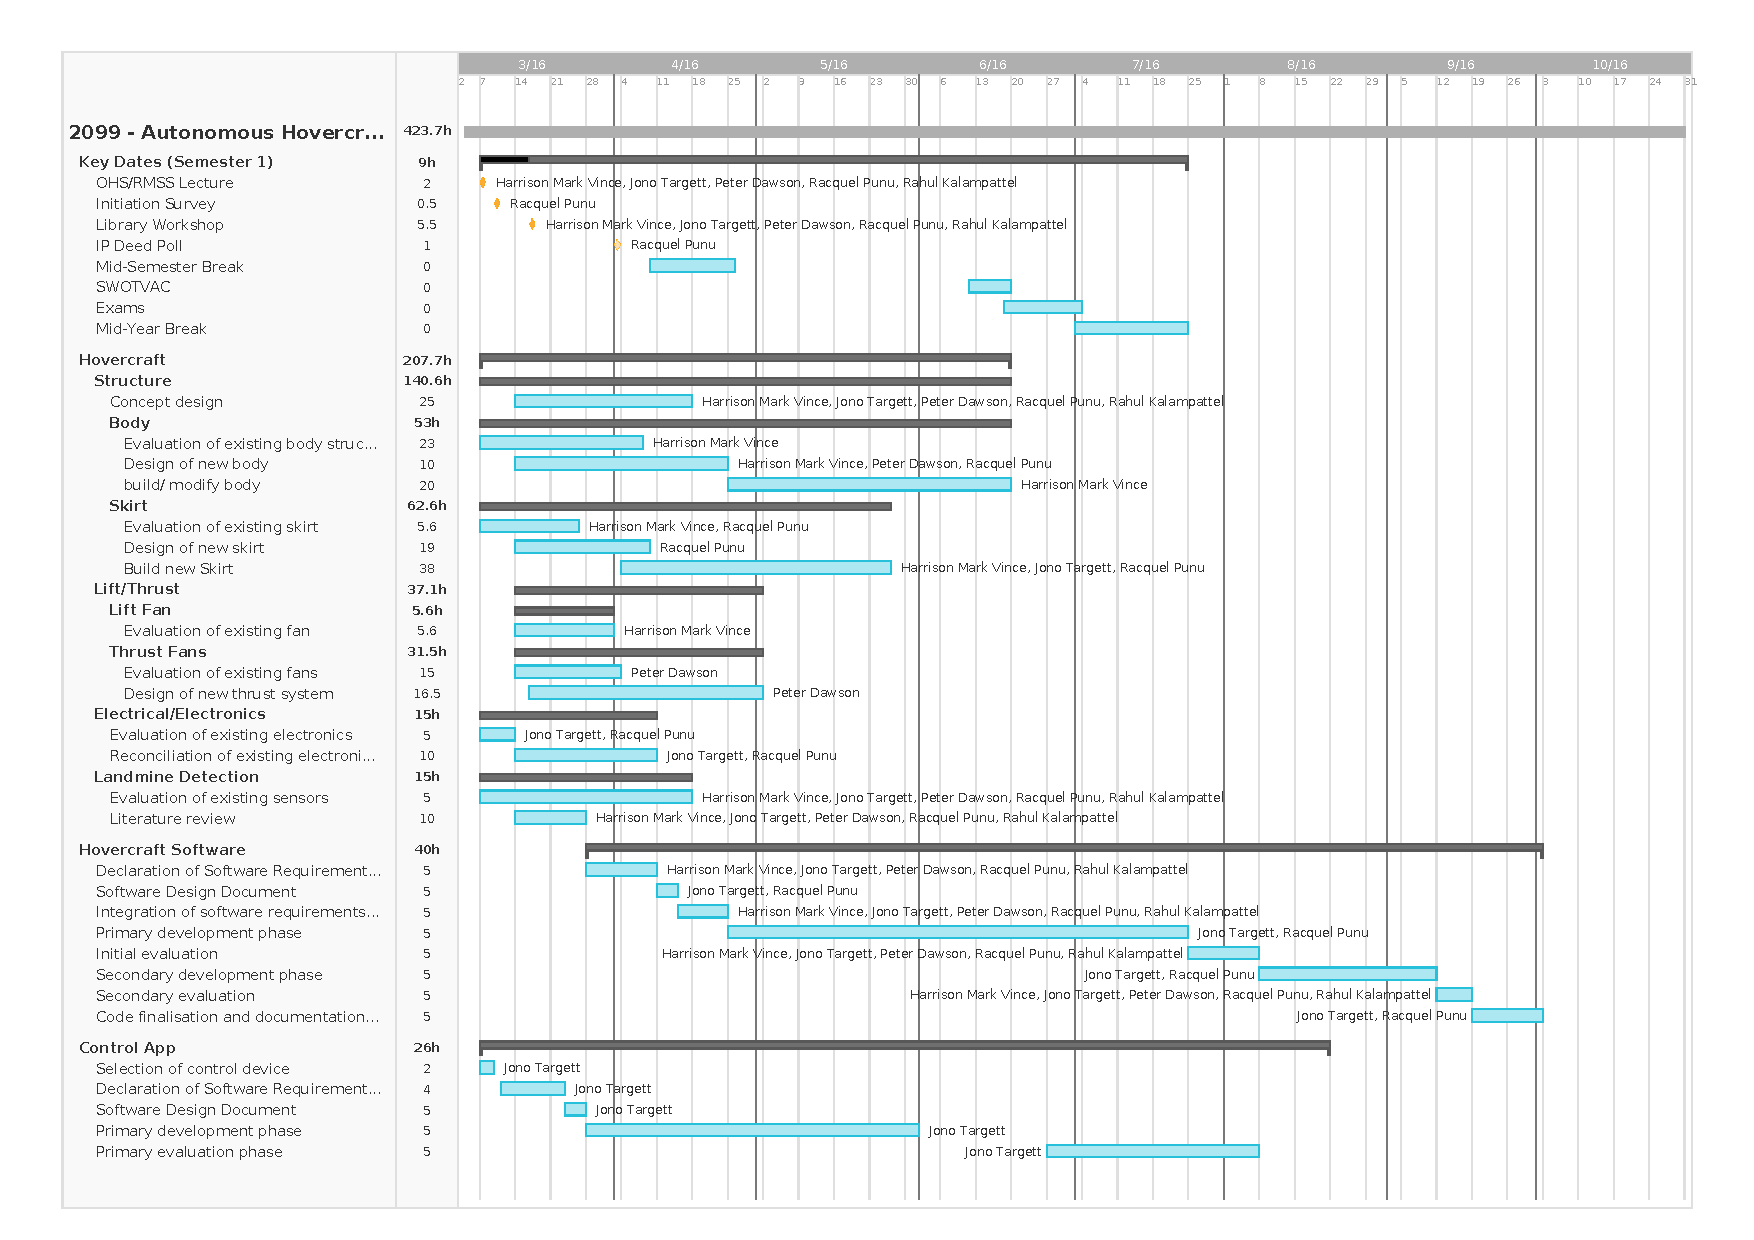
\includepdf[pages={1-},landscape]{8-Appendices/oldGantt.pdf}
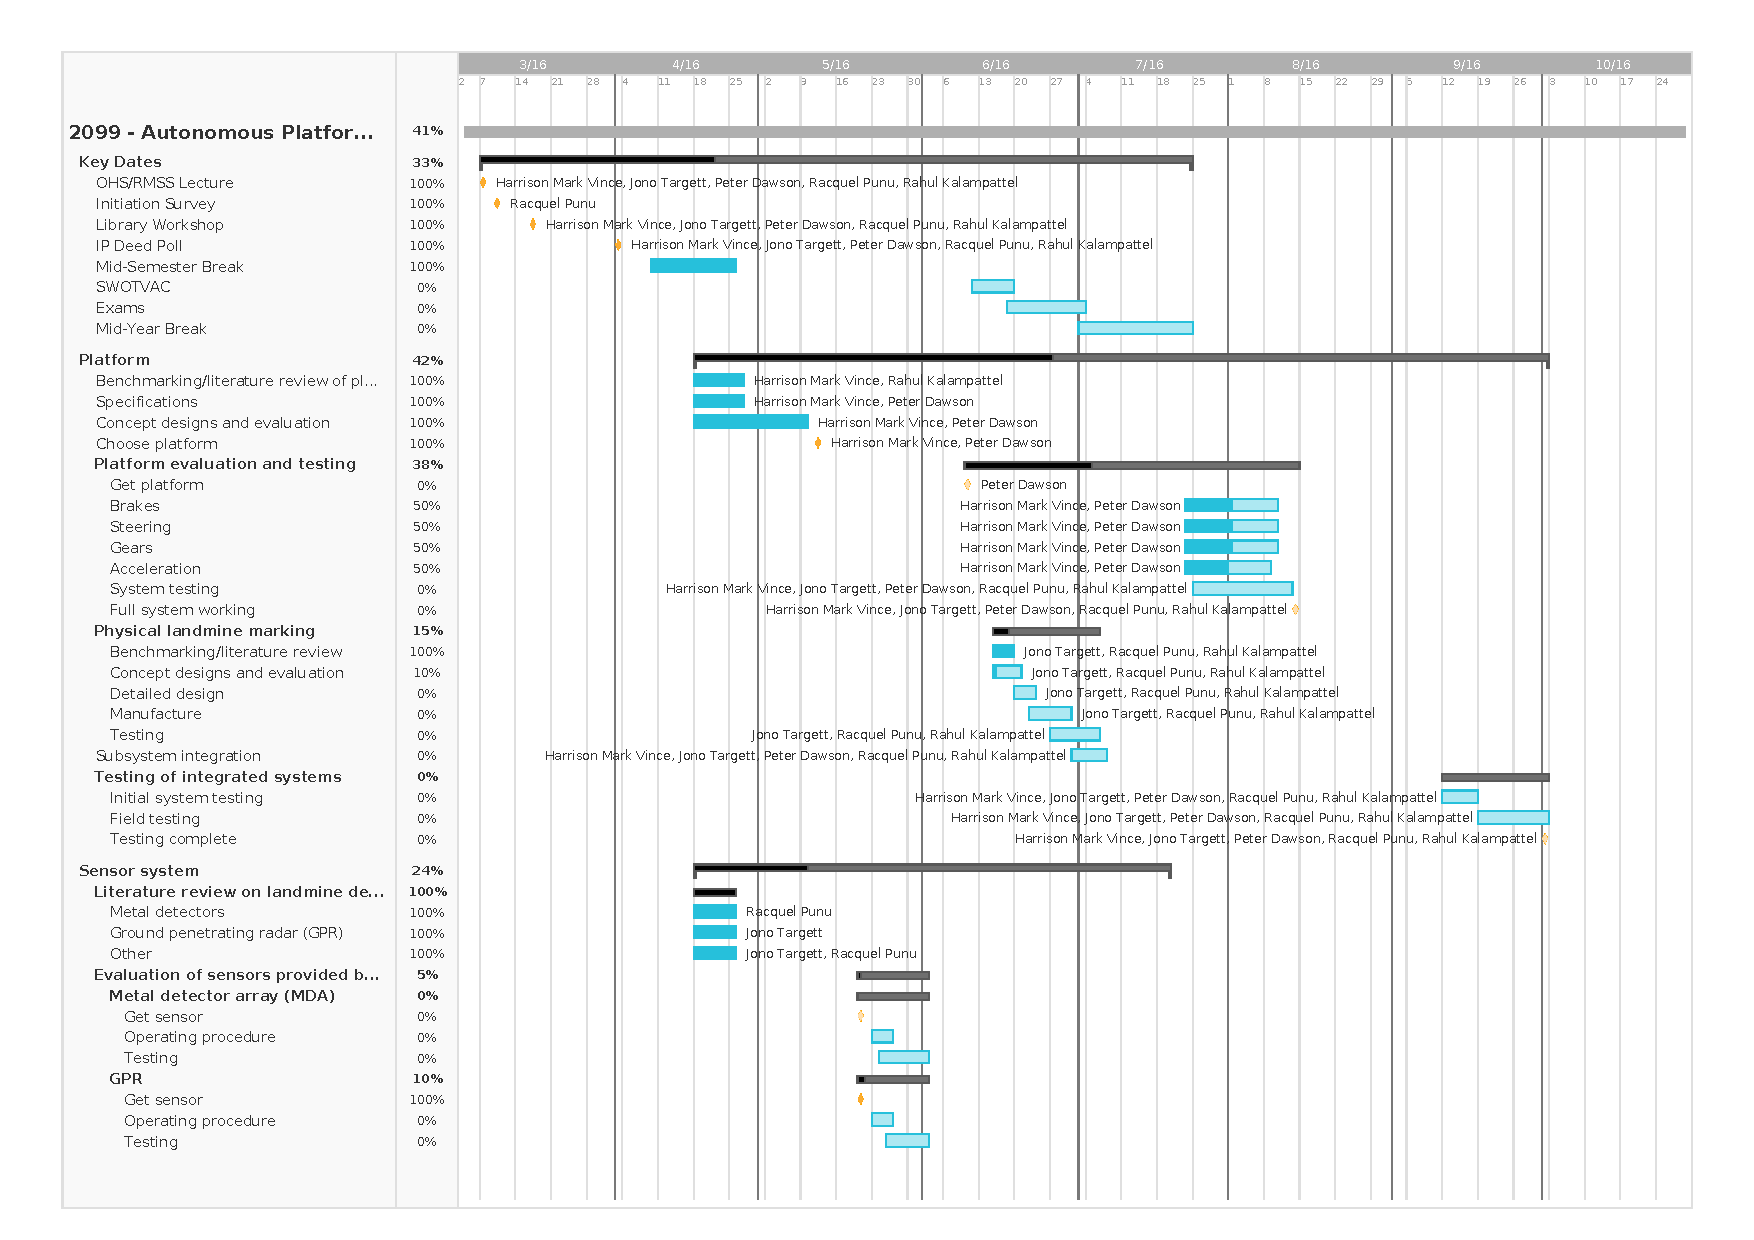
\includepdf[pages={1-},landscape]{8-Appendices/newGantt.pdf}

\chapter{Safety Documents}
\chaplabel{riskAss}
As part of the formal risk management for the project, a risk assessment must be carried out using the RMSS system, and a safe operating  procedure (SOP) must be developed. Both of these items, as discussed in \secref{safety}, are attached on the following pages.
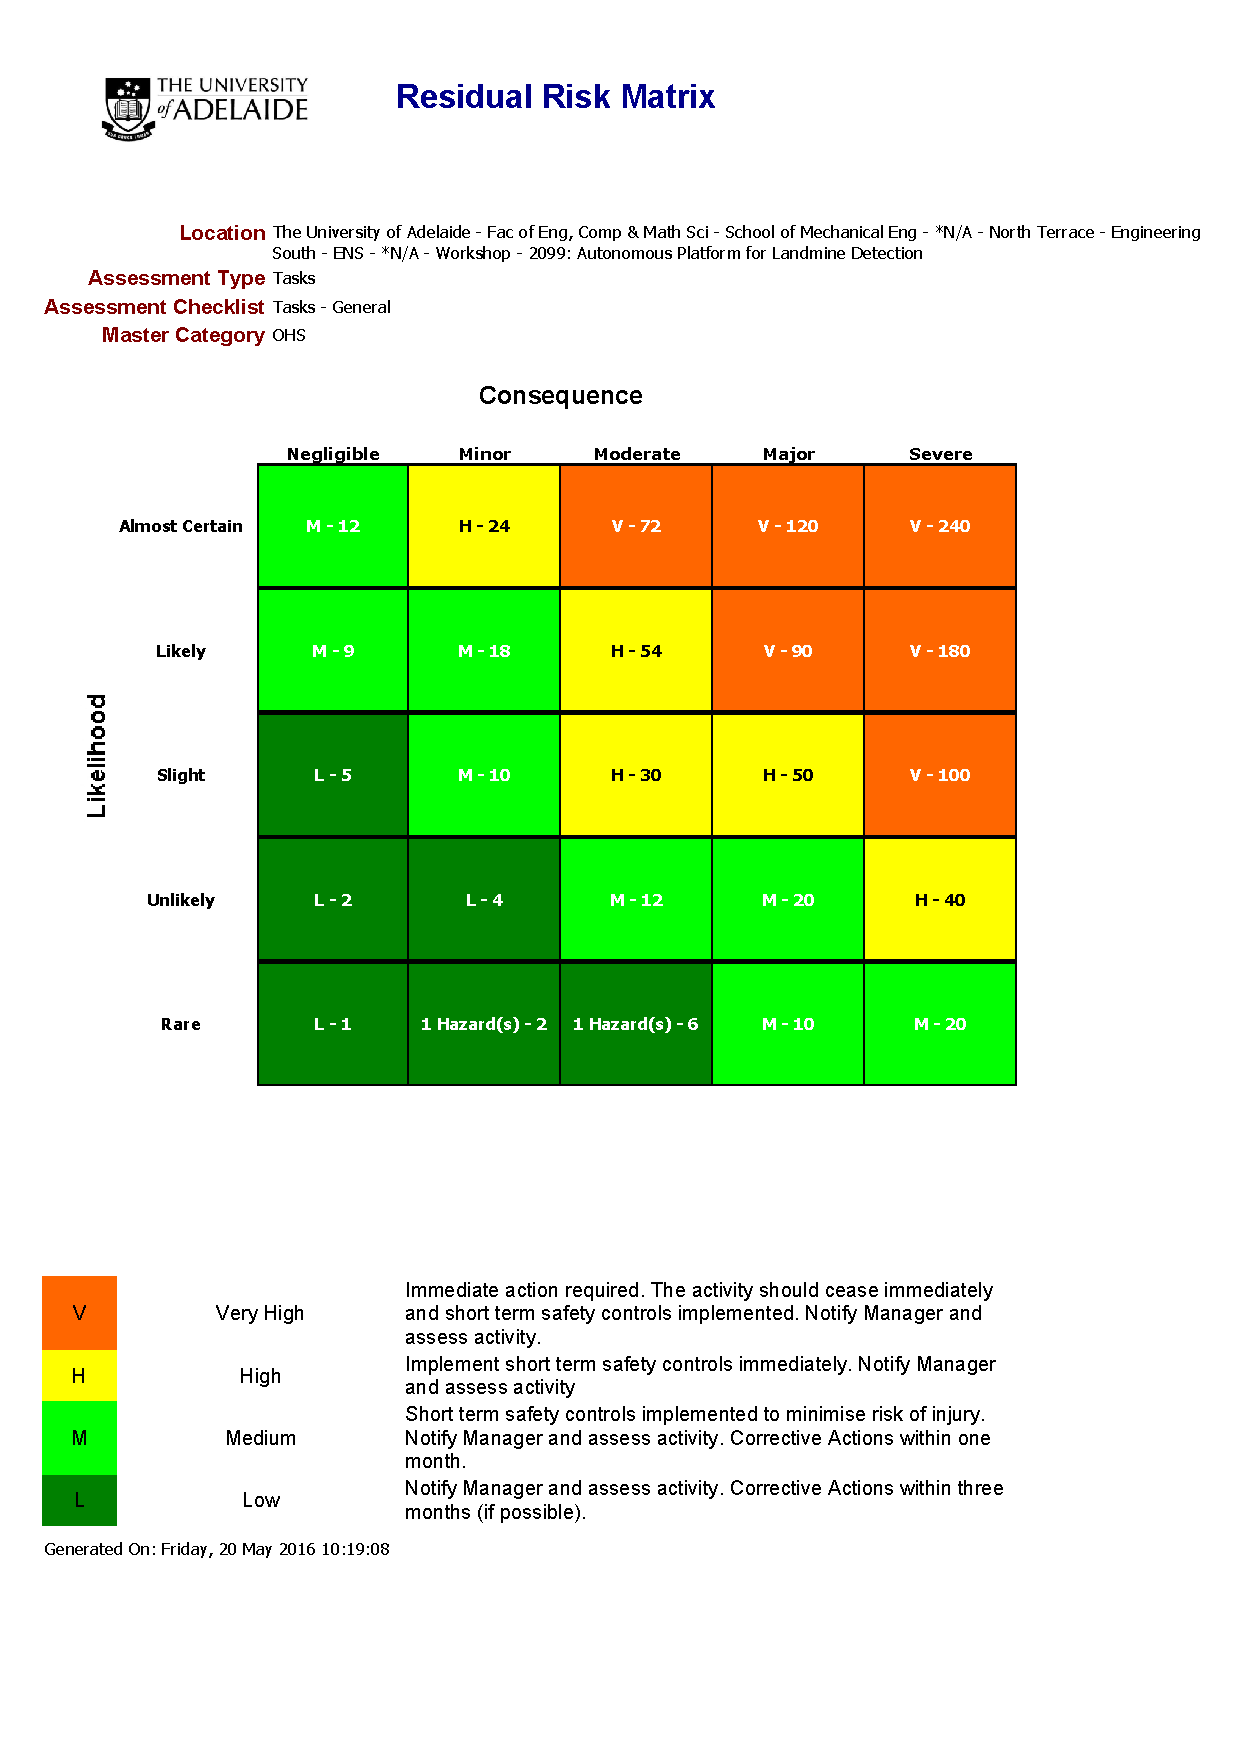
\includepdf{8-Appendices/residualRiskMatrix.pdf}
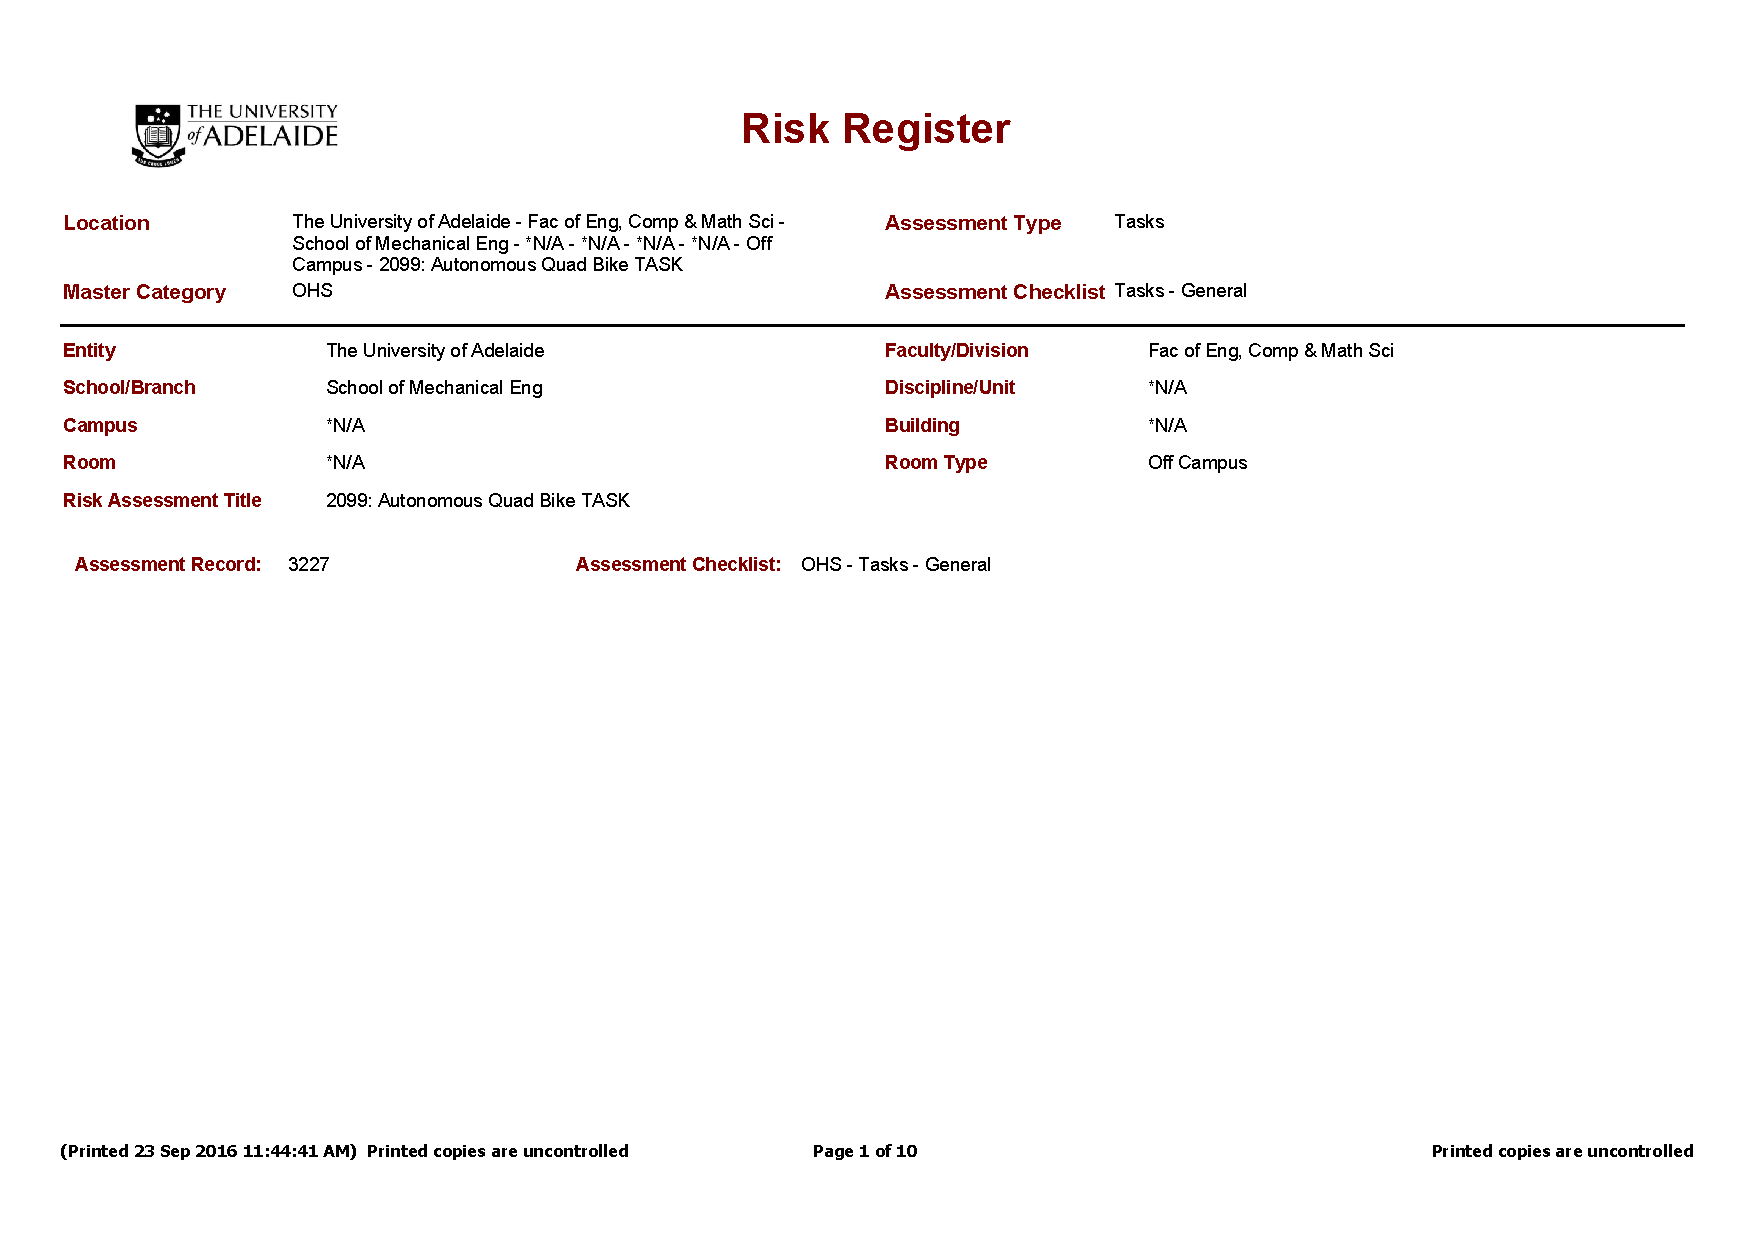
\includepdf[pages={1,3},landscape]{8-Appendices/riskRegister.pdf}
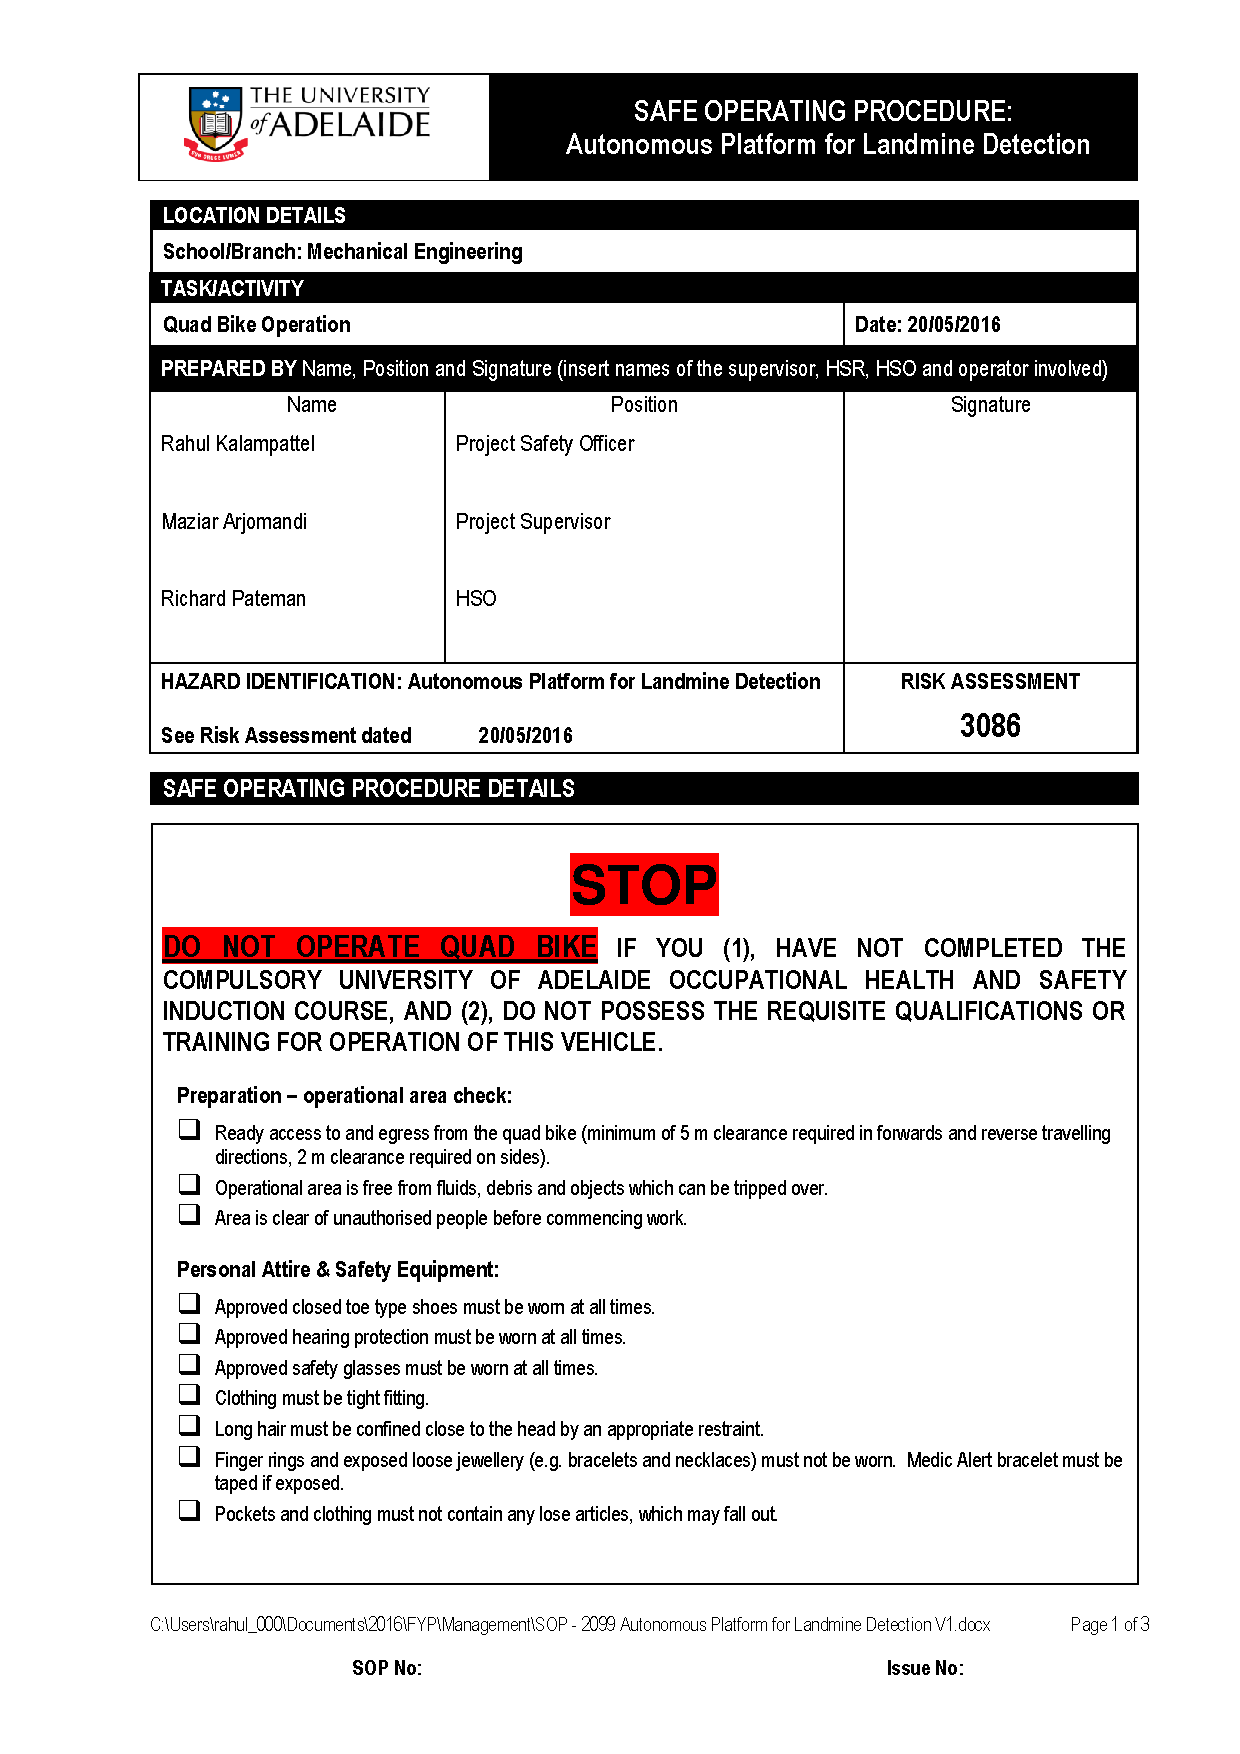
\includepdf[pages={1-}]{8-Appendices/SOP.pdf}

\chapter{Risks of Project Failure}
\chaplabel{riskFailureApp}
The risks to project failure are those events that may result in the project objectives not being completed. The risk level associated with an event is found by using the risk matrix, \Tabref{riskmatrix}.

\begin{table}[ht]
\caption{Risk matrix} \tablabel{riskmatrix}
\begin{tabular}{C{0.22\textwidth} C{0.22\textwidth} C{0.22\textwidth} C{0.22\textwidth}}
\toprule
\multicolumn{1}{c}{} & \multicolumn{3}{c}{\textbf{Impact}}\\ \cmidrule{2-4}
\textbf{Likelihood}&Minor&Moderate&Major\\ \midrule
Likely&\cellcolor{Yellow}Medium&\cellcolor{BurntOrange}High&\cellcolor{red}Extreme\\ 
Possible&\cellcolor{LimeGreen}Low&\cellcolor{Yellow}Medium&\cellcolor{BurntOrange} High\\ 
Unlikely&\cellcolor{OliveGreen}Negligible&\cellcolor{LimeGreen}Low&\cellcolor{Yellow}Medium\\ \bottomrule
\end{tabular}
\end{table}

\nohyphens{	% Stop hyphenation in table
\begin{longtable}{L{0.3\textwidth} L{0.1\textwidth} L{0.5\textwidth}}
\caption{Risk consequences, controls and recovery methods} \tablabel{risks}\\ \toprule
\textbf{Event} & \textbf{Risk} & \textbf{Consequences, controls and recovery}\\ \midrule\endfirsthead
\caption[]{Risk Consequences, Controls and Recovery Methods (continued)}\\ \toprule
\textbf{Event} & \textbf{Risk} & \textbf{Consequences, controls and recovery}\\ \midrule\endhead 

\multicolumn{1}{L{0.3\textwidth}}{\textbf{Existing platform unable to meet operational requirements}
The quad bike and associated hardware may not be sufficient to meet the performance specifications or achieve the project objectives} & \multicolumn{1}{L{0.1\textwidth}}{\cellcolor{Yellow}Medium} & \multicolumn{1}{L{0.5\textwidth}}{If the hardware on the quad bike does not function as well as required, it will be difficult to control the vehicle remotely, and even more difficult to automate. This will affect the entire system during the integrated testing stages of the project. In order to ensure that this does not become an issue later on, all aspects of quad bike will be tested and evaluated as soon as it is available. Necessary components will be serviced or replaced, and in the event that the extent of repairs is too large, sufficient funding is available to purchase a new platform.} \\ \midrule

\multicolumn{1}{L{0.3\textwidth}}{\textbf{Unable to successfully find targets}
The multi-sensor system may not be able to detect and confirm mines with a sufficient confidence level} & \multicolumn{1}{L{0.1\textwidth}}{\cellcolor{Yellow}Medium} & \multicolumn{1}{L{0.5\textwidth}}{Limited target detection and confirmation ability is likely to be due to difficulties encountered during signal processing and data fusion. This would mean the project goal could not be met. To reduce the likelihood of this occurring, a detailed plan has been devised for software development and testing. The multi-sensor system will only be tested once the performance of the individual sensor systems has been confirmed. In the event that the confidence level is still too low, simulated data can be used, allowing the testing of other related systems, such as the GPS logging system.} \\ \midrule

\multicolumn{1}{L{0.3\textwidth}}{\textbf{Automation and navigation cannot be achieved} Unable to operate the quad bike autonomously due to complexity, part failure or poor time management} & \multicolumn{1}{L{0.1\textwidth}}{\cellcolor{Yellow}Medium} & \multicolumn{1}{L{0.5\textwidth}}{Controlling the platform remotely is not anticipated to be a difficult task. Full automation of the system, to the level required for operation, carries increased risk due to complexity of the control software. To ensure that automation can be implemented successfully, control systems will be developed with a milestone based approach, whereby lower-level and simpler controls are implemented before more complex systems are commenced. Additionally, the software will be tested using a virtual platform.} \\ \midrule

\multicolumn{1}{L{0.3\textwidth}}{\textbf{Systems cannot be integrated}
Unable to use the sensor system in conjunction with the autonomous platform, either due to mounting issues or challenges with software} & \multicolumn{1}{L{0.1\textwidth}}{\cellcolor{LimeGreen}Low} & \multicolumn{1}{L{0.5\textwidth}}{An inability to integrate systems correctly will hinder testing, meaning the  project objective cannot be realised. Due to the small size and relatively insensitive nature of the sensors to disturbances, mounting will not be difficult. The high level software architecture will be developed in a way that allows for easy integration of systems. If any one of the component systems does not lend itself well to integration, its performance can be simulated.} \\ \midrule

\multicolumn{1}{L{0.3\textwidth}}{\textbf{Unable to find time to complete project}
Automating the platform, signal processing of sensor data and testing and integration prove too time consuming to manage with other commitments} & \multicolumn{1}{L{0.1\textwidth}}{\cellcolor{LimeGreen}Low} & \multicolumn{1}{L{0.5\textwidth}}{Not having enough sufficient time will mean that many of the objectives will not be completed. The likelihood of this occurring is reduced through effective project planning, i.e. the use of a Gantt chart, which enforces deadlines for individual tasks, hence reducing the possibility of failure. In the event that an individual is unable to complete a task, another member of the group will assist where possible.} \\ \midrule

\multicolumn{1}{L{0.3\textwidth}}{\textbf{Platform sustains damage or fails}
The quad bike is damaged during testing or undergoes structural, mechanical or electrical component failure} & \multicolumn{1}{L{0.1\textwidth}}{\cellcolor{LimeGreen}Low} & \multicolumn{1}{L{0.5\textwidth}}{If the quad bike is to crash, individual parts or the sensor payload may suffer damage. The quad bike could also injure an individual. The likelihood of this event is reduced by the fact that the platform will be travelling at low speeds, and the impact to the vehicle is reduced since it is designed for off-road use. Furthermore, an emergency stop switch and remote kill switch has been put in place as control measures. According to the SOP, inspections will be made before commencing operation, to make sure that the sensor payload is attached correctly. If the failure is of an electrical nature, directional control or autonomous capabilities may be lost. The likelihood of this occurring is small, however in the event that it does, parts can be replaced relatively easily and cheaply.} \\ \midrule

\multicolumn{1}{L{0.3\textwidth}}{\textbf{Unable to acquire parts in time}
Necessary parts for the control system, or replacement parts, are delayed} & \multicolumn{1}{L{0.1\textwidth}}{\cellcolor{LimeGreen}Low} & \multicolumn{1}{L{0.5\textwidth}}{If the delivery of parts takes too long, individual subsystems will be put behind schedule, as will the testing schedule of the entire platform. The likelihood of this is reduced through early research and selection of required parts, allowing for sufficient delivery time. In the event that parts do not arrive due to unforeseen circumstances, they can be substituted with available parts that may be of a similar specification.} \\ \bottomrule
\end{longtable}}
\newpage
\newgeometry{left=0.75in, right=0.75in, top=0.9in, bottom=0.8in}

%
%% 
%%% DON'T FORGET TO CHANGE THE GEOMETRY LATER
%%
%

\chapter{Budget Breakdown}
\chaplabel{budgetApp}
A detailed breakdown of the budget is provided in the following tables. \Tabref{expenditureCurrent} outlines current expenditure while \Tabref{expenditureFuture} summarises the expected expenditure for the remainder of the project. \Tabref{labourHours} provides a monthly breakdown of the hours spent on the project by each student and the associated costs. Salaries are calculated at the rate of \$26/hr, with other direct and indirect costs included. Direct costs incur an additional 30\% on top of salary for items such as superannuation, payroll tax, workcover, long service leave, etc. Indirect costs incur an additional 130\% on top of salary for items such as administration and tech support, infrastructure, rent, phone, internet, etc.
\nohyphens{	% Stop hyphenation in table
\begin{longtable}{L{0.20\textwidth} L{0.52\textwidth} L{0.18\textwidth}}
\caption{Current expenditure as at 01-06-2016} \tablabel{expenditureCurrent}\\ \toprule
\textbf{Subsystem} & \textbf{Item} & \textbf{Cost (\$)} \\ \midrule\endfirsthead 
\caption[]{Current Expenditure (continued)}\\ \toprule
\textbf{Subsystem} & \textbf{Item} & \textbf{Cost (\$)} \\ \midrule\endhead
\textbf{Electronics} & 10 Ft Mic Lead & 19.95 \\
& XLR/USB Converter Plug & 39.95\\
& Wireless-N Network Adapter & 20.00\\
& Wired Desktop (Keyboard + Mouse) & 19.00\\
& Samsung 120GB SSD & 69.00\\ \midrule
\multicolumn{2}{r}{\textbf{TOTAL}} & 167.90 \\ \bottomrule 
\end{longtable}}

\nohyphens{	% Stop hyphenation in table
\begin{longtable}{L{0.20\textwidth} L{0.52\textwidth} L{0.18\textwidth}}
\caption{Projected expenditure as at 01-06-2016} \tablabel{expenditureFuture}\\ \toprule
\textbf{Subsystem} & \textbf{Item} & \textbf{Cost (\$)} \\ \midrule\endfirsthead 
\caption[]{Projected Expenditure (continued)}\\ \toprule
\textbf{Subsystem} & \textbf{Item} & \textbf{Cost (\$)} \\ \midrule\endhead
\textbf{Structure} & Actuators (upgrade/replace) & 1,500 \\ 
& Service/Oil Change & 200 \\
& Sensor Mount & 340 \\ \midrule

\textbf{Sensors} & Ground Penetrating Radar unit & Supplied by the DSTG \\
& Metal Detector & 600\\ \midrule

\textbf{Power} & Petrol & 300 \\
& Batteries & 500 \\ \midrule

\textbf{Electronics} & Computer Upgrades & 500 \\ 
& 2 x GPS (H B Differential) & 450 \\ 
& IMU & 50 \\ 
& Microcontroller & 150 \\ 
& 9 Axis Accelerometer, Gyro, Magnetometer & 50 \\ 
& Licenses/Software & 100 \\ 
& GPS and Control Board & 200 \\ 
& Camera & 300 \\
& Receiver/Transmitter & 300 \\
& Test Mines & 100 \\
& Misc Electronics & 350 \\ \midrule

\multicolumn{2}{r}{\textbf{TOTAL}} & 5,990 \\ \bottomrule 
\end{longtable}}

\nohyphens{	% Stop hyphenation in table
\begin{longtable}{L{0.22\textwidth-2\tabcolsep}*{5}{L{0.12\textwidth-2\tabcolsep}} L{0.13\textwidth-2\tabcolsep}}
\caption{Breakdown of hours and costs (as at 01-06-2016)} \tablabel{labourHours}\\ \toprule
\textbf{Team Member} & \textbf{Harrison} & \textbf{Jono} & \textbf{Peter} & \textbf{Racquel} & \textbf{Rahul} & \textbf{Total} \\ \midrule\endfirsthead 
\caption[]{Breakdown of Hours and Cost (continued)}\\ \toprule
\textbf{Team Member} & \textbf{Jono} & \textbf{Harrison} & \textbf{Peter} & \textbf{Racquel} & \textbf{Rahul} & \textbf{Total} \\ \midrule\endhead 
\textbf{Hours} \\
\textbf{February} & - & - & - & 1.5 & 8 & 9.5 \\ 
\textbf{March} & 39.5 & 51.5 & 43 & 50.75 & 58 & 242.75 \\
\textbf{April} & 41.25 & 33 & 33.5 & 37.75 & 39 & 184.5 \\ 
\textbf{May} & 51.75 & 42.5 & 29.5 & 59.5 & 56.5 & 239.75 \\
\textbf{Total} & 132.5 & 127 & 106 & 149.5 & 161.5 & 676.5 \\ \midrule
\textbf{Wages} \\
\textbf{Total (Salary)} & \$3445.00 & \$3302.50 & \$2756.00 & \$3887.00 & \$4199.00 & \$17589.00 \\
\textbf{Total (Direct)} & \$1033.50 & \$990.60 & \$826.80 & \$1166.10 & \$1259.70 & \$5276.70 \\
\textbf{Total (Indirect)} & \$4478.50 & \$4292.60 & \$3582.80 & \$5053.10 & \$5458.70 & \$18657.60 \\
\textbf{Total Cost} & \$8957.00 & \$8585.20 & \$7165.60 & \$10106.20 & \$10917.40 & \$45731.40 \\ \midrule
\multicolumn{6}{r}{\textbf{Total Labour}} & \$45731.40 \\ \bottomrule
\end{longtable}}

\end{appendices}
\end{document}